\documentclass[10pt,oneside,onecolumn,openany,final]{memoir}
\setstocksize{11in}{8.5in}

\usepackage[toc,lot,lof]{multitoc}
\usepackage[top=.5in, bottom=.5in, left=.75in, right=.75in]{geometry}
\usepackage{graphicx} \graphicspath{{./images/}}
\usepackage{longtable}
\usepackage{mdwlist}
\usepackage{microtype} \DisableLigatures{encoding = *, family = *}
\usepackage{multicol}
\usepackage{textcomp}
\usepackage[normalem]{ulem}
\usepackage{wrapfig}
\usepackage{xtab}
\usepackage{enumerate}
\usepackage{phonetic}
\usepackage{bbding}
\usepackage{linearb}
\usepackage{cypriot}
\usepackage{tipa}
\usepackage{xfrac}
\usepackage{appendix}
\usepackage{xparse}
\usepackage{letltxmacro}
\usepackage{makeidx} \makeindex
\usepackage[table,dvipsnames]{xcolor}
\definecolor{offyellow}{RGB}{255,255,128}
\definecolor{links}{RGB}{200,0,50}
\usepackage{placeins}
\usepackage{floatflt}
\usepackage{anyfontsize}
\usepackage{colortbl}
\usepackage{tabularx}

\usepackage{longtable}
\usepackage{tabu}
\usepackage{afterpage}

%% Font
\usepackage[T1]{fontenc}
\usepackage[bitstream-charter]{mathdesign}
\usepackage{aurical}

\usepackage[colorlinks=true,linkcolor=blue,urlcolor=links,pdfstartview={XYZ null null 1.00},bookmarksdepth=2]{hyperref}
%%%%%%%%%%%%%%%%%%%%%%%%%
%%%% End of Import tion %%%%%%%%%%%
%%%%%%%%%%%%%%%%%%%%%%%%%

%%%%%%%%%%%%%%%%%%%%%%%%%%%%%%%%%%%%%%%%%%%%%%%%%%
%%%%%%%%%%%%%%%%%%%%%%%%%%%%%%%%%%%%%%%%%%%%%%%%%%
%%% Revised Commands
%%%%%%%%%%%%%%%%%%%%%%%%%%%%%%%%%%%%%%%%%%%%%%%%%%
%%%%%%%%%%%%%%%%%%%%%%%%%%%%%%%%%%%%%%%%%%%%%%%%%%
\makeatletter

%fiddles with how chapter titles are displayed
\renewcommand{\@makechapterhead}[1]{%
\vspace*{0 pt}{%
\raggedright \normalfont \fontsize{32}{32} \selectfont \bfseries%
\ifnum \value{secnumdepth}>-1%
  \if@mainmatter \vspace{-8pt} {\fontsize{20}{20} \selectfont Chapter \thechapter:}\\[8pt]%
  \fi%
\fi
\hspace{0.65cm} #1\par\nobreak\vspace{20 pt}%
}}

%makes paragraphs show up closer together
\renewcommand{\paragraph}{%
\@startsection{paragraph}{4}%
{\z@}{1.0ex \@plus 1ex \@minus 0.2ex}{-1em} % wtf is an 'ex' anyways?
{\normalfont\normalsize\bfseries}%
}

%lets multicolumn have the proper background colors as defined by rowcolors
\let\oldmc\multicolumn
\newcommand{\mcinherit}{% Activate \multicolumn inheritance
  \renewcommand{\multicolumn}[3]{%
    \oldmc{##1}{##2}{\ifodd\rownum \@oddrowcolor\else\@evenrowcolor\fi ##3}%
  }}

\makeatother

%add labels within sections, subsections, and subsubsections
\LetLtxMacro{\oldsection}{\section}
\renewcommand{\section}[1]{\oldsection{#1}\label{sec:#1}}

\LetLtxMacro{\oldsubsection}{\subsection}
\renewcommand{\subsection}[1]{\oldsubsection{#1}\label{sec:#1}}

\LetLtxMacro{\oldsubsubsection}{\subsubsection}
\renewcommand{\subsubsection}[1]{\oldsubsubsection{#1}\label{sec:#1}}

%only put chapters and sections into the TOC
\setcounter{secnumdepth}{1}
%makes a subsubsection start off indented.
\setlength{\beforesubsubsecskip}{-\beforesubsubsecskip}

%%%%%%%%%%%%%%%%%%%%%%%%%%%%%%%%%%%%%%%%%%%%%%%%%%
%%%%%%%%%%%%%%%%%%%%%%%%%%%%%%%%%%%%%%%%%%%%%%%%%%
%%% Table Formatting
%%%%%%%%%%%%%%%%%%%%%%%%%%%%%%%%%%%%%%%%%%%%%%%%%%
%%%%%%%%%%%%%%%%%%%%%%%%%%%%%%%%%%%%%%%%%%%%%%%%%%
\newcolumntype{L}[1]{>{\raggedright\let\newline\\\arraybackslash\hspace{0pt}}m{#1}} %New type of column 'L' that is ragged-right, behaves like a paragraph, and allows manual definition of width like a 'p' column.
\newcolumntype{C}[1]{>{\centering\let\newline\\\arraybackslash\hspace{0pt}}m{#1}}  %New type of column 'C' that is centered, behaves like a paragraph, and allows manual definition of width like a 'p' column.
\newcolumntype{R}[1]{>{\raggedleft\let\newline\\\arraybackslash\hspace{0pt}}m{#1}}  %New type of column 'R' that is ragged-left, behaves like a paragraph, and allows manual definition of width like a 'p' column.
\newcommand{\header}{\rowcolor{headercolor}}
%when inserted in a row, makes that row the color headercolor

%%%%%%%%%%%%%%%%%%%%%%%%%%%%%%%%%%%%%%%%%%%%%%%%%%
%%%%%%%%%%%%%%%%%%%%%%%%%%%%%%%%%%%%%%%%%%%%%%%%%%
%%% New Commands
%%%%%%%%%%%%%%%%%%%%%%%%%%%%%%%%%%%%%%%%%%%%%%%%%%
%%%%%%%%%%%%%%%%%%%%%%%%%%%%%%%%%%%%%%%%%%%%%%%%%%

%%%%%%%%%%%%%%%%%%%%%%%%
%%Basic Formatting
%%%%%%%%%%%%%%%%%%%%%%%%
\newcommand{\originallineskip}{\baselineskip}
 %A command that is equal to the original \baselineskip of the doc, in case we change it for a section and want to change it back later
\newcommand{\ability}[2]{\smallskip%\noindent 
 \textbf{#1} #2} 
%The \ability{#1}{#2} command from legacy-source. Should rarely be directly used, changes to this will cascade into other new commands that use its functionality
\newcommand{\itemspace}{\setlength{\itemsep}{-1mm}\setlength{\topsep}{-1mm} }
%A command from legacy-source for compatabilty
\newcommand{\listone}{\begin{list}{$\bullet$}{\itemspace}}
%A type of list from legacy sorce
\newcommand{\listnum}{\begin{list}{\textbf{\arabic{counter}}:}{\usecounter{counter}}}
\newcommand{\spell}[1]{\emph{\MakeLowercase{#1}}}
%makes spell name lowercase italics.
\setlength{\parindent}{0pt}

%%%%%%%%%%%%%%%%%%%%%%%%
%%Logic
%%%%%%%%%%%%%%%%%%%%%%%%
\newcommand{\testempty}{\empty}
\newcommand{\isempty}{\empty}
%Two commands that can be compared to one another for \ifx logic tests. \isempty should never be changed. If \testempty holds a value of anything but empty, the test should return false.
\newcounter{counter}

%%%%%%%%%%%%%%%%%%%%%%%%
%%Colors
%%%%%%%%%%%%%%%%%%%%%%%%
\colorlet{colorone}{white}
\colorlet{colortwo}{gray!15}
\colorlet{headercolor}{gray!50}
\colorlet{tablecolorone}{gray!40}
\colorlet{tablecolortwo}{gray!20}

%%%%%%%%%%%%%%%%%%%%%%%%
%%Sectioning
%%%%%%%%%%%%%%%%%%%%%%%%
\newcommand{\classentry}[1]{\newpage \section{#1} \renewcommand{\class}{#1} \index{#1 (class)} \renewcommand{\testempty}{\isempty}}
%Starts a new page, creates a section with the name of the class (#1), sets \class to be the name of the class, indexes the class.
\newcommand{\raceentry}[1]{\oldsection{#1}\index{#1 (race)}\label{race:#1}}

\newcommand{\Requirements}{\oldsubsubsection*{Requirements}}

\newcommand{\Basics}{\oldsubsubsection*{Basics}}

\newcommand{\ClassFeatures}{\oldsubsubsection*{Class Features}}

\newcommand{\skillentry}[2]{\oldsubsection[#1]{#1 #2}\index{#1 (skill)}\label{skill:#1}}

%%%%%%%%%%%%%%%%%%%%%%%%
%%Class Chapter
%%%%%%%%%%%%%%%%%%%%%%%%
\newcommand{\class}{placeholder}
%Holds the classes name, as defined by \classentry

\newcommand{\quot}[1]{
	\vspace{-8pt}
	\noindent\emph{#1}\medskip}
%Displays a flavor quote.}

\newenvironment{classpreamble}{
\renewcommand\tabularxcolumn[1]{m{##1}}
\center
\rowcolors{1}{colorone}{colortwo}
\tabularx{\textwidth}{X}
}{
\endtabularx
\endcenter
\renewcommand\tabularxcolumn[1]{p{##1}}
}

\newcommand{\desc}[1]{  #1 \\}
\newcommand{\playingaclass}[1]{\ability{Playing a \class :}{#1}\\}
\newcommand{\hitdie}[1]{\ability{Hit Die:}{#1}\\}
\newcommand{\alignment}[1]{\ability{Alignment:}{#1}\\}
\newcommand{\races}[1]{\ability{Races:}{#1}\\}
\newcommand{\startinggold}[1]{\ability{Starting Gold:}{#1}\\}
\newcommand{\startingage}[1]{\ability{Starting Age:}{#1}\\}  
\newcommand{\skillpoints}[1]{\ability{Skill Points per Level:}{#1 + Intelligence Bonus}\\}
\newcommand{\classskills}[1]{\ability{Class Skills:}{The {\class}'s class skills (and the key ability for each skill) are #1}\\}

\newcommand{\startclassfeatures}{
 \smallskip\noindent All of the following are class features of the \class ~class.}
%place before actual class features entries.

\newcommand{\proficiencies}[1]{
 \ability{Weapon and Armor Proficiencies:}{The \class ~is proficient with #1}}
%Displays proficiencies with minimal input, implimentation looks like \proficiencies{the proficiencies}

\newcommand{\classfeature}[2]{
  \ability{#1}{#2}}
%No functional difference from \ability currently

%%%%Class Table Commands

\newcommand{\gbab}{\empty}
\newcommand{\mbab}{\empty}
\newcommand{\fort}{\empty}
\newcommand{\refl}{\empty}
\newcommand{\will}{\empty}
%Creates new commands for use in \ifx statements for formatting purposes.

\newcommand{\goodbab}{\renewcommand{\gbab}{\empty}\renewcommand{\mbab}{a}}
\newcommand{\modebab}{\renewcommand{\gbab}{a}\renewcommand{\mbab}{\empty}}
\newcommand{\poorbab}{\renewcommand{\gbab}{a}\renewcommand{\mbab}{a}}
%A set of commands to tell LaTeX what BAB progression the class has. Only one should be called per class.

\newcommand{\goodfor}{\renewcommand{\fort}{\empty}}
\newcommand{\poorfor}{\renewcommand{\fort}{a}}
%A set of commands to tell LaTeX what Fortitude progression the class has. Only one should be called per class.

\newcommand{\goodref}{\renewcommand{\refl}{\empty}}
\newcommand{\poorref}{\renewcommand{\refl}{a}}
%A set of commands to tell LaTeX what Reflex progression the class has. Only one should be called per class.

\newcommand{\goodwil}{\renewcommand{\will}{\empty}}
\newcommand{\poorwil}{\renewcommand{\will}{a}}
%A set of commands to tell LaTeX what Will progression the class has. Only one should be called per class.

\newenvironment{classtable}[1]
{
\table[htb]
\center
\rowcolors{1}{colorone}{colortwo}
\tabularx{\textwidth}{p{.275in}lp{0.275in}p{0.275in}p{0.275in}Xllll}
\rowcolor{headercolor} Level & Base Attack & Fort. & Ref. & Will & Special #1\\
}{
\endtabularx
\endcenter
\endtable
}
%A a new environment that sets up the class tables. Include the \level commands between \begin{classtable}.

\newenvironment{minorcastingclasstable}
{
\table[htb]
\center
\rowcolors{1}{colorone}{colortwo}
\tabularx{\textwidth}{p{.275in}lp{0.275in}p{0.275in}p{0.275in}Xccccccc}
\rowcolor{headercolor} & & & & & &\multicolumn{7}{c}{Spells Per Day (By Level)} \\
\rowcolor{headercolor} Level & Base Attack & Fort. & Ref. & Will & Special &0&1&2&3&4&5&6\\
}{
\endtabularx
\endcenter
\endtable
}
%A a new environment similar to classtable, but with columns for a minor (zero through six) spell slot progression.

\newenvironment{fullcastingclasstable}
{
\table[htb]
\center
\rowcolors{1}{colorone}{colortwo}
\tabularx{\textwidth}{p{.275in}lp{0.275in}p{0.275in}p{0.275in}Xcccccccccc}
\rowcolor{headercolor} & & & & & &\multicolumn{10}{c}{Spells Per Day (By Level)} \\
\rowcolor{headercolor} Level & Base Attack & Fort. & Ref. & Will & Special &0&1&2&3&4&5&6&7&8&9\\
}{
\endtabularx
\endcenter
\endtable
}
%Another environment for class tables, this one for full (0 through 9) spell slot progression.

\newcommand{\levelone}[1]{
1st  & \ifx\gbab\isempty +1 \else\ifx\mbab\isempty +0 \else +0 \fi \fi
	 & \ifx\fort\isempty +2 \else +0 \fi
	 & \ifx\refl\isempty +2 \else +0 \fi
	 & \ifx\will\isempty +2 \else +0 \fi
	 & #1 \\}
%A command that declares a table row within the class feature table.

\newcommand{\leveltwo}[1]{
2nd  & \ifx\gbab\isempty +2 \else\ifx\mbab\isempty +1 \else +1 \fi \fi
	 & \ifx\fort\isempty +3 \else +0 \fi
	 & \ifx\refl\isempty +3 \else +0 \fi
	 & \ifx\will\isempty +3 \else +0 \fi
	 & #1 \\}
%A command that declares a table row within the class feature table.

\newcommand{\levelthree}[1]{
3rd  & \ifx\gbab\isempty +3 \else\ifx\mbab\isempty +2 \else +1 \fi \fi
	 & \ifx\fort\isempty +3 \else +1 \fi
	 & \ifx\refl\isempty +3 \else +1 \fi
	 & \ifx\will\isempty +3 \else +1 \fi
	 & #1 \\}
%A command that declares a table row within the class feature table.

\newcommand{\levelfour}[1]{
4th  & \ifx\gbab\isempty +4 \else\ifx\mbab\isempty +3 \else +2 \fi \fi
	 & \ifx\fort\isempty +4 \else +1 \fi
	 & \ifx\refl\isempty +4 \else +1 \fi
	 & \ifx\will\isempty +4 \else +1 \fi
	 & #1 \\}
%A command that declares a table row within the class feature table.

\newcommand{\levelfive}[1]{
5th  & \ifx\gbab\isempty +5 \else\ifx\mbab\isempty +3 \else +2 \fi \fi
	 & \ifx\fort\isempty +4 \else +1 \fi
	 & \ifx\refl\isempty +4 \else +1 \fi
	 & \ifx\will\isempty +4 \else +1 \fi
	 & #1 \\}
%A command that declares a table row within the class feature table.
	 
\newcommand{\levelsix}[1]{
6th  & \ifx\gbab\isempty +6/+1 \else\ifx\mbab\isempty +4 \else +3 \fi \fi
	 & \ifx\fort\isempty +5 \else +2 \fi
	 & \ifx\refl\isempty +5 \else +2 \fi
	 & \ifx\will\isempty +5 \else +2 \fi
	 & #1 \\}
%A command that declares a table row within the class feature table.

\newcommand{\levelseven}[1]{
7th  & \ifx\gbab\isempty +7/+2 \else\ifx\mbab\isempty +5 \else +3 \fi \fi
	 & \ifx\fort\isempty +5 \else +2 \fi
	 & \ifx\refl\isempty +5 \else +2 \fi
	 & \ifx\will\isempty +5 \else +2 \fi
	 & #1 \\}
%A command that declares a table row within the class feature table.
	 
\newcommand{\leveleight}[1]{
8th  & \ifx\gbab\isempty +8/+3 \else\ifx\mbab\isempty +6/+1 \else +4 \fi \fi
	 & \ifx\fort\isempty +6 \else +2 \fi
	 & \ifx\refl\isempty +6 \else +2 \fi
	 & \ifx\will\isempty +6 \else +2 \fi
	 & #1 \\}
%A command that declares a table row within the class feature table.
	 
\newcommand{\levelnine}[1]{
9th  & \ifx\gbab\isempty +9/+4 \else\ifx\mbab\isempty +6/+1 \else +4 \fi \fi
	 & \ifx\fort\isempty +6 \else +3 \fi
	 & \ifx\refl\isempty +6 \else +3 \fi
	 & \ifx\will\isempty +6 \else +3 \fi
	 & #1 \\}
%A command that declares a table row within the class feature table.
	 
\newcommand{\levelten}[1]{
10th & \ifx\gbab\isempty +10/+5 \else\ifx\mbab\isempty +7/+2 \else +5 \fi \fi
	 & \ifx\fort\isempty +7 \else +3 \fi
	 & \ifx\refl\isempty +7 \else +3 \fi
	 & \ifx\will\isempty +7 \else +3 \fi
	 & #1 \\}
%A command that declares a table row within the class feature table.
	 
\newcommand{\leveleleven}[1]{
11th & \ifx\gbab\isempty +11/+6/+6 \else\ifx\mbab\isempty +8/+3 \else +5 \fi \fi
	 & \ifx\fort\isempty +7 \else +3 \fi
	 & \ifx\refl\isempty +7 \else +3 \fi
	 & \ifx\will\isempty +7 \else +3 \fi
	 & #1 \\}
%A command that declares a table row within the class feature table.
	 
\newcommand{\leveltwelve}[1]{
12th & \ifx\gbab\isempty +12/+7/+7 \else\ifx\mbab\isempty +9/+4 \else +6/+1 \fi \fi
	 & \ifx\fort\isempty +8 \else +4 \fi
	 & \ifx\refl\isempty +8 \else +4 \fi
	 & \ifx\will\isempty +8 \else +4 \fi
	 & #1 \\}
%A command that declares a table row within the class feature table.
	 
\newcommand{\levelthirteen}[1]{
13th & \ifx\gbab\isempty +13/+8/+8 \else\ifx\mbab\isempty +9/+4 \else +6/+1 \fi \fi
	 & \ifx\fort\isempty +8 \else +4 \fi
	 & \ifx\refl\isempty +8 \else +4 \fi
	 & \ifx\will\isempty +8 \else +4 \fi
	 & #1 \\}
%A command that declares a table row within the class feature table.
	 
\newcommand{\levelfourteen}[1]{
14th & \ifx\gbab\isempty +14/+9/+9 \else\ifx\mbab\isempty +10/+5 \else +7/+2 \fi \fi
	 & \ifx\fort\isempty +9 \else +4 \fi
	 & \ifx\refl\isempty +9 \else +4 \fi
	 & \ifx\will\isempty +9 \else +4 \fi
	 & #1 \\}
%A command that declares a table row within the class feature table.
	 
\newcommand{\levelfifteen}[1]{
15th & \ifx\gbab\isempty +15/+10/+10 \else\ifx\mbab\isempty +11/+6/+6 \else +7/+2 \fi \fi
	 & \ifx\fort\isempty +9 \else +5 \fi
	 & \ifx\refl\isempty +9 \else +5 \fi
	 & \ifx\will\isempty +9 \else +5 \fi
	 & #1 \\}
%A command that declares a table row within the class feature table.
	 
\newcommand{\levelsixteen}[1]{
16th & \ifx\gbab\isempty +16/+11/+11/+11 \else\ifx\mbab\isempty +12/+7/+7 \else +8/+3 \fi \fi
	 & \ifx\fort\isempty +10 \else +5 \fi
	 & \ifx\refl\isempty +10 \else +5 \fi
	 & \ifx\will\isempty +10 \else +5 \fi
	 & #1 \\}
%A command that declares a table row within the class feature table.
	 
\newcommand{\levelseventeen}[1]{
17th & \ifx\gbab\isempty +17/+12/+12/+12 \else\ifx\mbab\isempty +12/+7/+7 \else +8/+3 \fi \fi
	 & \ifx\fort\isempty +10 \else +5 \fi
	 & \ifx\refl\isempty +10 \else +5 \fi
	 & \ifx\will\isempty +10 \else +5 \fi
	 & #1 \\}
%A command that declares a table row within the class feature table.
	 
\newcommand{\leveleighteen}[1]{
18th & \ifx\gbab\isempty +18/+13/+13/+13 \else\ifx\mbab\isempty +13/+8/+8 \else +9/+4 \fi \fi
	 & \ifx\fort\isempty +11 \else +6 \fi
	 & \ifx\refl\isempty +11 \else +6 \fi
	 & \ifx\will\isempty +11 \else +6 \fi
	 & #1 \\}
%A command that declares a table row within the class feature table.
	 
\newcommand{\levelnineteen}[1]{
19th & \ifx\gbab\isempty +19/+14/+14/+14 \else\ifx\mbab\isempty +14/+9/+9 \else +9/+4 \fi \fi
	 & \ifx\fort\isempty +11 \else +6 \fi
	 & \ifx\refl\isempty +11 \else +6 \fi
	 & \ifx\will\isempty +11 \else +6 \fi
	 & #1 \\}
%A command that declares a table row within the class feature table.
	 
\newcommand{\leveltwenty}[1]{
20th & \ifx\gbab\isempty +20/+15/+15/+15 \else\ifx\mbab\isempty +15/+10/+10 \else +10/+5 \fi \fi
	 & \ifx\fort\isempty +12 \else +6 \fi
	 & \ifx\refl\isempty +12 \else +6 \fi
	 & \ifx\will\isempty +12 \else +6 \fi
	 & #1 \\}
%A command that declares a table row within the class feature table.

%\newmdenv[hidealllines=true,backgroundcolor=gray!20]{optionbox}
%A new environemnt, abilty box, that gets redefined by other commands later, notably to produce color backgrounds for classes

\newenvironment{optional}[2]{
   \renewcommand\tabularxcolumn[1]{m{##1}}
   \begin{tabularx}{\textwidth}{X}
   \rowcolor{headercolor}\textbf{#1} \\
   \ifx#2\isempty\else#2 \\
   \end{tabularx}
}{
\renewcommand\tabularxcolumn[1]{p{##1}}
}

\newcommand{\option}[2]{
\begin{tabularx}{\textwidth}{X}
\rowcolor{colortwo} #1 \\
\end{tabularx}
#2
~\\*
}

%%%%%%%%%%%%%%%%%%%%%%%%
%%Unsorted Commands
%%%%%%%%%%%%%%%%%%%%%%%%
\newcommand{\tagline}[1]{\vspace{-6pt} \textit{#1} \medskip}

\newcommand{\gameterm}[1]{#1\index{#1}}

\NewDocumentCommand\featentry{m+g}{%
  \IfNoValueTF{#2}
    {\oldsubsubsection[#1]{#1 [General]}\label{feat:#1}}%no second arg, general feat
    {\oldsubsubsection[#1]{#1 [#2]}\label{feat:#1}}%second arg, special type of feat
}

\newcommand{\spellentry}[1]{\oldsubsubsection{#1}\label{spell:#1}}

\NewDocumentCommand\linkrace{m+g}{%
  \IfNoValueTF{#2}
    {\hyperref[race:#1]{#1}}%no second arg, display is same as link
    {\hyperref[race:#1]{#2}}%second arg, link to first and display second
}
\NewDocumentCommand\linkclass{m+g}{%
  \IfNoValueTF{#2}
    {\hyperref[class:#1]{#1}}%no second arg, display is same as link
    {\hyperref[class:#1]{#2}}%second arg, link to first and display second
}
\NewDocumentCommand\linkskill{m+g}{%
  \IfNoValueTF{#2}
    {\hyperref[skill:#1]{#1}}%no second arg, display is same as link
    {\hyperref[skill:#1]{#2}}%second arg, link to first and display second
}
\NewDocumentCommand\linkfeat{m+g}{%
  \IfNoValueTF{#2}
    {\hyperref[feat:#1]{#1}}%no second arg, display is same as link
    {\hyperref[feat:#1]{#2}}%second arg, link to first and display second
}
\NewDocumentCommand\linkspell{m+g}{%
  \IfNoValueTF{#2}
    {\hyperref[spell:#1]{#1}}%no second arg, display is same as link
    {\hyperref[spell:#1]{#2}}%second arg, link to first and display second
}
\NewDocumentCommand\linkcondition{m+g}{%
  \IfNoValueTF{#2}
    {\hyperref[condition:#1]{#1}}%no second arg, display is same as link
    {\hyperref[condition:#1]{#2}}%second arg, link to first and display second
}
\NewDocumentCommand\linkability{m+g}{%
  \IfNoValueTF{#2}
    {\hyperref[ability:#1]{#1}}%no second arg, display is same as link
    {\hyperref[ability:#1]{#2}}%second arg, link to first and display second
}
\NewDocumentCommand\linksec{m+g}{%
  \IfNoValueTF{#2}
    {\hyperref[sec:#1]{#1}}%no second arg, display is same as link
    {\hyperref[sec:#1]{#2}}%second arg, link to first and display second
}

\begin{document}

%%%%%%%%%%%%%%%%%%%%%%%%%%%%%%%%%%%%%%%%%%%%%%%%%%
%%%%%%%%%%%%%%%%%%%%%%%%%%%%%%%%%%%%%%%%%%%%%%%%%%
%%% Title Page
%%%%%%%%%%%%%%%%%%%%%%%%%%%%%%%%%%%%%%%%%%%%%%%%%%
%%%%%%%%%%%%%%%%%%%%%%%%%%%%%%%%%%%%%%%%%%%%%%%%%%
\thispagestyle{empty}
\begin{center}
\textsc{\Large}\\[0.25cm]
\rule{\linewidth}{0.5mm} \\[0.70cm]
\fontsize{30}{30} \selectfont Tome Reference Document\\[.30cm]
\fontsize{16}{18} \selectfont \guillemotleft{} For that game we all known and love \guillemotright{}\\
\rule{\linewidth}{0.5mm} \\[0.6cm]
%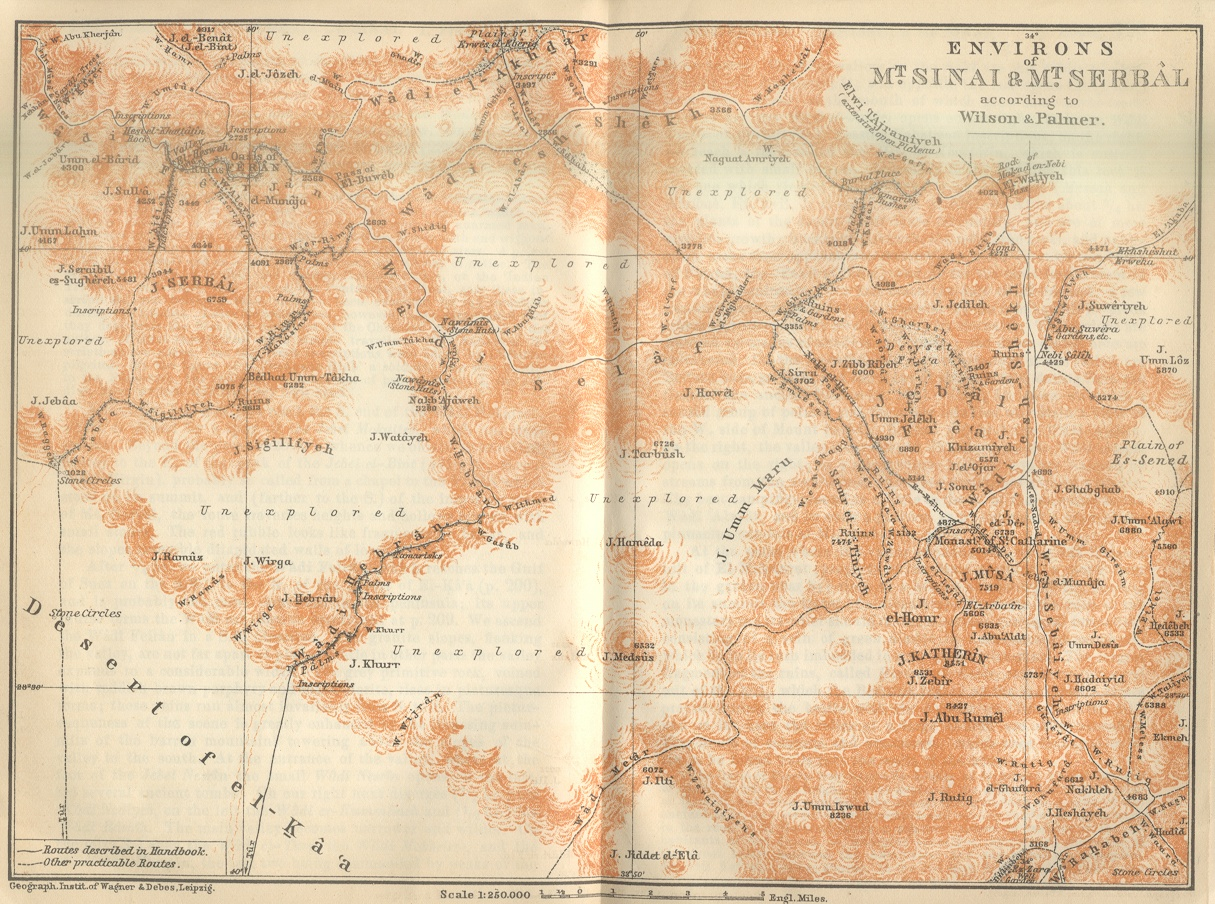
\includegraphics[clip,trim=5cm 2cm 9cm 1cm,width=\linewidth]{OldBookArt--MapImages-173.jpg}
\vfill
{\large \textit{This material is Open Game Content, and is licensed for public use under the terms of the Open Game License v1.0a.}\\
\today}
\end{center}

\pagebreak
\sffamily
\pagestyle{plain}
\raggedbottom

%%%%%%%%%%%%%%%%%%%%%%%%%%%%%%%%%%%%%%%%%%%%%%%%%%
%%%%%%%%%%%%%%%%%%%%%%%%%%%%%%%%%%%%%%%%%%%%%%%%%%
%%% Table of Contents
%%%%%%%%%%%%%%%%%%%%%%%%%%%%%%%%%%%%%%%%%%%%%%%%%%
%%%%%%%%%%%%%%%%%%%%%%%%%%%%%%%%%%%%%%%%%%%%%%%%%%
\renewcommand{\contentsname}{Table of Contents}
\setcounter{tocdepth}{1}
\tableofcontents

%%%%%%%%%%%%%%%%%%%%%%%%%%%%%%%%%%%%%%%%%%%%%%%%%%
%%%%%%%%%%%%%%%%%%%%%%%%%%%%%%%%%%%%%%%%%%%%%%%%%%
%%% Main Content
%%%%%%%%%%%%%%%%%%%%%%%%%%%%%%%%%%%%%%%%%%%%%%%%%%
%%%%%%%%%%%%%%%%%%%%%%%%%%%%%%%%%%%%%%%%%%%%%%%%%%

%% Primary Chapters Here

\clearpage

\chapter{Introduction}
\section{What is a Role-playing Game?}
foo
\section{What You Need To Play}
foo
\section{The Core Mechanic}
foo
\section{Creating a Character}
foo

\chapter{Races}
\section{Race Basics}
foo
\section{Drow}
foo
\section{Dwarf}
foo
\section{Elf}
foo
\section{Gnome}
foo
\section{Goblin}
foo
\section{Half-Elf}
foo
\section{Halfling}
foo
\section{Hobgoblin}
foo
\section{Human}
foo
\section{Kobold}
foo
\section{Orc}
foo

\chapter{Classes}
\section{Class Basics}
foo

\classname{Assassin} \label{class:assassin}
\vspace{-8pt}
\quot{"I kill people. Individually, you are a person. Collectively, I think you count as people."}

\desc{An assassin is a master of the art of killing, a vicious weapon honed by experience and inclination to learn the myriad ways to end a life. Unlike common warriors or rogues, an Assassin does not study various fighting arts or muddle his training with martial dirty tricks, he instead studies the anatomy of the various creatures of wildly different anatomies and forms of existence, and he uses this knowledge to place his blows in areas vital for biological or mystical reasons. Stealth and sudden violence are his hallmarks, and various exotic tools and killing methods become his tools.}

\desc{While most societies consider assassination to be a vile art, or at best a dishonorable or unvalorous one, the reasons that drive these killers vary. Cold-hearted mercenaries share a skill set with dedicated demon-hunters, differing only in the application of their skills. Only the most na\"ive student of ethics believes that all killing is evil, or that nobility cannot be found in a mercifully quick death.}

\ability{Alignment:}{An Assassin may be of any alignment.}

\ability{Races:}{Any}

\ability{Starting Gold:}{6d4x10 gp (150 gold)}

\ability{Starting Age:}{As Rogue.}

\ability{Hit Die:}{d6}

\ability{Class Skills:}{The Assassin's skills (and the key ability for each skill) are Balance (Dex), Bluff (Cha), Climb (Str), Concentration (Con), Craft (Int), Diplomacy (Cha), Disable Device (Int), Disguise (Cha), Gather Information (Cha), Hide (Dex), Intimidate (Cha), Jump (Str), Knowledge (all) (Int), Listen (Wis), Move Silently (Dex), Perform (Cha), Profession (Wis), Search (Int), Sense Motive (Wis), Sleight of Hand (Dex), Spellcraft (Int), Spot (Wis), Swim (Str), Tumble (Dex), and Use Magic Device (Cha).}

\ability{Skills/Level:}{6 + Intelligence Bonus}

\begin{table}[htb]
\begin{small}
\begin{tabular}{lp{1.9cm}p{0.7cm}p{0.7cm}p{0.7cm}l}
Level  &Base Attack Bonus &Fort Save &Ref Save &Will Save &Special\\
1st &+0 &+2 &+2 &+0 &Poison Use, Death Attack +3d6, Personal Immunity, Spellcasting\\
2nd &+1 &+3 &+3 &+0 &Uncanny Dodge, Death Attack +4d6\\
3rd &+2 &+3 &+3 &+1 &Hide in Plain Sight, Death Attack +5d6\\
4th &+3 &+4 &+4 &+1 &Cloak of Discretion, Death Attack +6d6\\
5th &+3 &+4 &+4 &+1 &Traps, Trapmaking, Death Attack +7d6\\
6th &+4 &+5 &+5 &+2 &Palm Weapon, Death Attack +8d6\\
7th &+5 &+5 &+5 &+2 &Full Death Attack, Death Attack +9d6\\
8th &+6/+1 &+6 &+6 &+2 &Nerve of the Assassin, Death Attack +10d6\\
9th &+6/+1 &+6 &+6 &+3 &Improved Uncanny Dodge, Death Attack +11d6\\
10th &+7/+2 &+7 &+7 &+3 &Skill Mastery, Death Attack +12d6\\
11th &+8/+3 &+7 &+7 &+3 &Poisonmaster, Death Attack +13d6\\
12th &+8/+3 &+8 &+8 &+4 &Personal Immunity, Death Attack +14d6\\
13th &+9/+4 &+8 &+8 &+4 &Exotic Method, Death Attack +15d6\\
14th &+10/+5 &+9 &+9 &+4 &Personal Immunity, Death Attack +16d6\\
15th &+11/+6/+6 &+9 &+9 &+5 &Killer's Proof, Death Attack +17d6\\
16th &+12/+7/+7 &+10 &+10 &+5 &Exotic Method, Death Attack +18d6\\
17th &+12/+7/+7 &+10 &+10 &+5 &Death by a Thousand Cuts, Death Attack +19d6\\
18th &+13/+8/+8 &+11 &+11 &+6 &Mind Blank, Death Attack +20d6\\
19th &+14/+9/+9 &+11 &+11 &+6 &Exotic Method, Death Attack +21d6\\
20th &+15/+10/+10 &+12 &+12 &+6 &Killing Strike, Death Attack +22d6\\
\end{tabular}
\end{small}
\end{table}

\begin{floatingfigure}{3.9in}
\begin{small}
\noindent\begin{tabular}{lllllllllllllllll}
 & \multicolumn{7}{c}{Assassin Spells Per Day}  &   &\multicolumn{7}{c}{Assassin Spells Known}\\
  &0 &1 &2 &3 &4 &5 &6 &  &  &0 &1 &2 &3 &4 &5 &6\\
1 &2 &- &- &- &- &- &- &  &1 &4 &- &- &- &- &- &-\\
2 &3 &0 &- &- &- &- &- &  &2 &5 &2 &- &- &- &- &-\\
3 &3 &1 &- &- &- &- &- &  &3 &6 &3 &- &- &- &- &-\\
4 &3 &2 &0 &- &- &- &- &  &4 &6 &3 &2 &- &- &- &-\\
5 &3 &3 &1 &- &- &- &- &  &5 &6 &4 &3 &- &- &- &-\\
6 &3 &3 &2 &- &- &- &- &  &6 &6 &4 &3 &- &- &- &-\\
7 &3 &3 &2 &0 &- &- &- &  &7 &6 &4 &4 &2 &- &- &-\\
8 &3 &3 &3 &1 &- &- &- &  &8 &6 &4 &4 &3 &- &- &-\\
9 &3 &3 &3 &2 &- &- &- &  &9 &6 &4 &4 &3 &- &- &-\\
10 &3 &3 &3 &2 &0 &- &- &  &10 &6 &4 &4 &4 &2 &- &-\\
11 &3 &3 &3 &3 &1 &- &- &  &11 &6 &4 &4 &4 &3 &- &-\\
12 &3 &3 &3 &3 &2 &- &- &  &12 &6 &4 &4 &4 &3 &- &-\\
13 &3 &3 &3 &3 &2 &0 &- &  &13 &6 &4 &4 &4 &4 &2 &-\\
14 &3 &3 &3 &3 &3 &1 &- &  &14 &6 &4 &4 &4 &4 &3 &-\\
15 &3 &3 &3 &3 &3 &2 &- &  &15 &6 &4 &4 &4 &4 &3 &-\\
16 &3 &3 &3 &3 &3 &2 &0 &  &16 &6 &5 &4 &4 &4 &4 &2\\
17 &3 &3 &3 &3 &3 &3 &1 &  &17 &6 &5 &5 &4 &4 &4 &3\\
18 &3 &3 &3 &3 &3 &3 &2 &  &18 &6 &5 &5 &5 &4 &4 &3\\
19 &3 &3 &3 &3 &3 &3 &3 &  &19 &6 &5 &5 &5 &5 &4 &4\\
20 &3 &3 &3 &3 &3 &3 &3 &  &20 &6 &5 &5 &5 &5 &5 &4\\
\end{tabular}
\end{small}
\end{floatingfigure}

\smallskip\noindent All of the following are Class Features of the Assassin class.

\ability{Weapon and Armor Proficiency:}{Assassins are proficient with all Light Weapons, as well as simple weapons, repeating crossbows, and hand crossbows. At first level, an Assassin gains proficiency with one Exotic Weapon of her choice. Assassins are proficient with Light Armor but not with shields.}

\ability{Spellcasting:}{The Assassin is an Arcane Spellcaster with the same spells per day and spells known progression as a Bard, except that he gains no more than three spell slots per level. An Assassin's spells known may be chosen from the Sorcerer/Wizard list, and must be from the schools of Divination, Illusion, or Necromancy. To cast an Assassin spell, she must have an Intelligence at least equal to 10 + the Spell level. The DC of the Assassin's spells is Intelligence based and the bonus spells are Intelligence based.}

\ability{Poison Use (Ex):}{An Assassin may prepare, apply, and use poison without any chance of poisoning herself.}

\ability{Death Attack (Ex):}{An Assassin may spend a full-round action to study an opponent who would be denied their Dexterity bonus if she instead attacked that target. If she does so, her next attack is a Death Attack if she makes it within 1 round. A Death Attack inflicts a number of extra dice of damage equal to her Assassin level plus two dice, but only if the target is denied its Dexterity Bonus to AC against that attack. Special attacks such as a coup de grace may be a Death Attack. Assassins are well trained in eliminating magical or distant opponents, and do not have to meet the stringent requirements of a sneak attack, though if a character has both sneak attack and death attack, they stack if the character meets the requirements of both. As long as the victim is denied their dexterity against attacks from the assassin during the study action and the attack itself, it counts as a death attack. An Assassin may load a crossbow simultaneously with his action to study his target if he has a Base Attack Bonus of +1 or more.}

\ability{Personal Immunity (Ex):}{Choose four poisons, an Assassin is immune to all four of those poisons, even if they are made available in a stronger strength. At levels 5, 7, and 12 the Assassin may choose one more type of poison to become immune to. At level 14, an Assassin becomes immune to all poisons.}

\ability{Uncanny Dodge (Ex):}{Starting at 2nd level, an Assassin can react to danger before his senses would normally allow him to do so. He retains her Dexterity bonus to AC (if any) even if she is caught flat-footed or struck by an invisible attacker. However, he still loses her Dexterity bonus to AC if immobilized. If an Assassin already has uncanny dodge from a different class he automatically gains improved uncanny dodge (see below) instead.}

\ability{Hide in Plain Sight (Ex):}{A 3rd level Assassin can hide in unusual locations, and may hide in areas without cover or concealment without penalty. An Assassin may even hide while being observed. This ability does not remove the -10 penalty for moving at full speed, or the -20 penalty for running or fighting.}

\ability{Cloak of Discretion (Su):}{At 4th level, an Assassin is protected by a constant \emph{nondetection} effect, with a caster level equal to his character level.}

\ability{Trapfinding:}{At 5th level, Assassins can use the Search skill to locate traps when the task has a Difficulty Class higher than 20. Finding a nonmagical trap has a DC of at least 20, or higher if it is well hidden. Finding a magic trap has a DC of 25 + the level of the spell used to create it. Assassins can use the Disable Device skill to disarm magic traps. A magic trap generally has a DC of 25 + the level of the spell used to create it. An Assassin who beats a trap's DC by 10 or more with a Disable Device check can study a trap, figure out how it works, and bypass it (with her party) without disarming it.}

\ability{Trapmaking:}{At 5th level, the Assassin learns to build simple mechanical traps in out of common materials. As long as has access to ropes, flexible material like green wood, and weapon-grade materials like sharpened wooden sticks or steel weapons, he can build an improvised trap in 10 minutes. He can build any non-magical trap on the "CR 1" trap list that doesn't involve a pit. These traps have a Search DC equal to 20 + the Assassin's level, have a BAB equal to his own, and are always single-use traps. He may add poison to these traps, if he has access to it, but it will dry out in an hour.}

\ability{Palm Weapon (Su):}{At 6th level, the Assassin learns to conceal weapons with supernatural skill. Any weapon successfully concealed with Sleight of Hand cannot be found with divination magic.}

\ability{Full Death Attack:}{At 7th level, if the Assassin studies an opponent to perform a Death Attack, she can make a full attack during the next round where every attack inflicts Death Attack damage as long as the target was denied their Dexterity bonus to AC against the first attack in the full attack action.}

\ability{Nerve of the Killer:}{At 8th level, an Assassin gains a limited immunity to compulsion and charm effects. While studying a target for a Death Attack, and for one round afterward, he counts as if he were within a \spell{protection from evil} effect. This does not confer a deflection bonus to AC.}

\ability{Improved Uncanny Dodge (Ex):}{An Assassin of 9th level or higher can no longer be flanked. This defense denies another character the ability to sneak attack the character by flanking him, unless the attacker has at least four more levels in a class that provides sneak attack than the target. If a character already has uncanny dodge (see above) from a second class, the character automatically gains improved uncanny dodge instead, and the levels from the classes that grant uncanny dodge stack to determine the minimum level required to flank the character.}

\ability{Skill Mastery (Ex):}{At 10th level, an Assassin becomes so certain in the use of certain skills that she can use them reliably even under adverse conditions. When making a skill check with Climb, Disable Device, Hide, Move Silently, Search, Spellcraft, Use Magic Device, Use Rope, or Swim, she may take 10 even if stress and distractions would normally prevent her from doing so.}

\ability{Poisonmaster:}{At 11th level, the Assassin learns alchemic secrets for creating short-term poisons. By expending an entire healer's kit worth of materials and an hour of time, he can synthesize one dose of any poison in the DMG. This poison degrades to uselessness in one week.}

\ability{Exotic Method:}{At 13th, 16th, and 19th level the Assassin learns an exotic form of killing from the list below. Once chosen, this ability does not change:}
\listone

    \item \ability{Carrier:}{Three times per day, the Assassin can cast \spell{contagion} as a swift action spell-like ability.}
    \item \ability{Poison of the Cockatrice:}{Twice per day, the Assassin can cast \spell{flesh to stone} as a swift action spell-like ability.}
    \item \ability{Killer Faerie Arts:}{Twice per day, the Assassin can cast \spell{polymorph other} as a swift action spell-like ability.}
    \item \ability{Proxy Assassin:}{Twice per day, the Assassin can cast \spell{summon monster VII} as a spell-like ability. This effect lasts 10 minutes.}
    \item \ability{Death By Plane:}{Once per day, the Assassin can cast \spell{plane shift} as a spell-like ability.}
    \item \ability{Dimesional Rip:}{Once per day, the Assassin can cast \spell{implosion} as a spell-like ability. The duration of this effect is three rounds.}
    \item \ability{New School:}{The Assassin may now choose spells known from a new school.}
\end{list}
\vspace{8pt}

\ability{Killer's Proof (Su):}{At 15th level, the Assassin learns to steal the souls of those he kills. If he is holding an onyx worth at least 100 GP when he kills an enemy, he may place their soul within the gem as if he has cast \spell{soul bind} on them at the moment of their death.}

\ability{Death by a Thousand Cuts:}{At 17th level, the assassin has learned to kill even the hardiest of foes by reducing their physical form to shambles. Every successful Death attack inflicts a cumulative -2 Dexterity penalty to the Assassin's victim. These penalties last one day.}

\ability{Mind Blank (Su):}{At 18th level, the Assassin is protected by a constant \spell{mind blank} effect.}

\ability{Killing Strike (Su):}{At 20th level, the Assassin's Death Attacks bypass his victim's DR and hardness.}


\classname{Barbarian} \label{class:barbarian}
\vspace{-8pt}
\quot{''My name is Sharptooth of the Wolf Tribe. Your women, lands, and riches are mine.''}

\ability{Playing a Barbarian:}{Playing a Barbarian is actually very easy. In general, you hit things, and they fall down. A Barbarian's action in almost any circumstance can plausibly be ''I hit it with my great axe!" As such, a Barbarian character can be a good method to introduce a new player to the game or kill some orcs when you've had a few glasses of brew.}

\ability{Alignment:}{Every alignment has its share of Barbarians, however more Barbarians are of Chaotic alignment than of Lawful Alignment.}

\ability{Races:}{Anybody can become a barbarian, and in areas with little in the way of civilization, a lot of people do.}

\ability{Starting Gold:}{4d6x10 gp (140 gold)}

\ability{Starting Age:}{As Barbarian.}

\ability{Hit Die:}{d12}

\ability{Class Skills:}{The Barbarian's class skills (and the key ability for each skill) are Balance (Dex), Climb (Str), Hide (Dex), Intimidate (Cha), Jump (Str), Knowledge: Nature (Int), Listen (Wis), Move Silently (Dex), Sense Motive (Wis), Spot (Wis), Survival (Wis), and Swim (Str).}

\ability{Skills/Level:}{4 + Intelligence Bonus}

\begin{table}[htb]
\begin{small}
\begin{tabular}{lp{3cm}p{0.7cm}p{0.7cm}p{0.7cm}l}
Level  &Base Attack Bonus &Fort Save &Ref Save &Will Save &Special\\
1st &+1 &+2 &+0 &+0 &Rage, Fast Healing 1\\
2nd &+2 &+3 &+0 &+0 &Rage Dice +1d6, Combat Movement +5'\\
3rd &+3 &+3 &+1 &+1 &Battle Hardened\\
4th &+4 &+4 &+1 &+1 &Rage Dice +2d6, Combat Movement +10'\\
5th &+5 &+4 &+1 &+1 &Sidestep Hazards , Fast Healing 5\\
6th &+6/+1 &+5 &+2 &+2 &Rage Dice +3d6, Combat Movement +15'\\
7th &+7/+2 &+5 &+2 &+2 &Great Blows\\
8th &+8/+3 &+6 &+2 &+2 &Rage Dice +4d6, Combat Movement +20'\\
9th &+9/+4 &+6 &+3 &+3 &Great Life\\
10th &+10/+5 &+7 &+3 &+3 &Rage Dice +5d6, Combat Movement +25', Fast Healing 10\\
11th &+11/+6/+6 &+7 &+3 &+3 &Call the Horde\\
12th &+12/+7/+7 &+8 &+4 &+4 &Rage Dice +6d6, Combat Movement +30'\\
13th &+13/+8/+8 &+8 &+4 &+4 &Watched by Totems\\
14th &+14/+9/+9 &+9 &+4 &+4 &Rage Dice +7d6, Combat Movement +35'\\
15th &+15/+10/+10 &+9 &+5 &+5 &Primal Assault, Fast Healing 15\\
16th &+16/+11/+11/+11 &+10 &+5 &+5 &Rage Dice +8d6, Combat Movement +40'\\
17th &+17/+12/+12/+12 &+10 &+5 &+5 &Savagery\\
18th &+18/+13/+13/+13 &+11 &+6 &+6 &Rage Dice +9d6, Combat Movement +45'\\
19th &+19/+14/+14/+14 &+11 &+6 &+6 &One With The Beast\\
20th &+20/+15/+15/+15 &+12 &+6 &+6 &Rage Dice +10d6, Combat Movement +50', Fast Healing 20\\
\end{tabular}
\end{small}
\end{table}

\smallskip\noindent All of the following are Class Features of the Barbarian class.


\ability{Weapon and Armor Proficiency:}{Barbarians are proficient with simple weapons, martial weapons, light armor, medium armor and with shields.}

\ability{Rage (Ex):}{When doing melee damage to a foe or being struck by a foe, a Barbarian may choose to enter a Rage as an immediate action. While Raging, a Barbarian gains a +2 morale bonus to hit and damage in melee combat and may apply any Rage Dice he has to his melee damage rolls. He also gains a +2 to saves, a -2 to AC, and he gains DR X/-- with ''X" being equal to half his Barbarian level +2 (rounded down). For example, a 1st level Barbarian has DR 3/-- while Raging and a 10th level Barbarian has DR 7/-- while Raging. While Raging, a Barbarian may not cast spells, activate magic items, use spell-like abilities, or drop his weapons or shield. Rage lasts until he has neither struck an enemy for three consecutive rounds nor suffered damage from an enemy for three consecutive rounds. He may voluntarily end a Rage as a full-round action.}

\ability{Fast Healing:}{Barbarians shrug off wounds that would cripple a lesser man, and have learned to draw upon deep reserves of energy and stamina. At 1st level, they gain Fast Healing 1. At 5th level this becomes Fast Healing 5, Fast Healing 10 at 10th level, Fast Healing 15 at 15th level, and Fast Healing 20 at 20th level. This healing only applies while he is not raging. \smallskip

If a Barbarian ever multiclasses, he permanently loses this ability. A multiclass character does not gain this ability.  A character with 4 or more levels of Barbarian gains this ability even if multiclassed.}

\ability{Rage Dice:}{While Raging, a Barbarian may add these dice of damage to each of his melee attacks. These dice are not multiplied by damage multipliers, and are not applied to any bonus attacks beyond those granted by Base Attack Bonus. These dice are not sneak attack dice, and do not count as sneak attack dice for the prerequisites of prestige classes or feats.}

\ability{Combat Movement:}{While Raging, a Barbarian moves faster in combat, and may add his Combat Movement to his speed when he takes a move action to move.}

\ability{Battle Hardened:}{At 3th level, a Raging Barbarian's mind has been closed off from distractions by the depths of his bloodlust and battle fury. While Raging, he may use his Fortitude Save in place of his Will Save. If he is under the effects of a compulsion or fear effect, he may act normally while Raging as if he was inside a \spell{protection from evil} effect.}

\ability{Sidestep Hazards (Ex):}{At 5th level, a Raging Barbarian learns to sidestep hazards with an intuitive and primal danger sense. While Raging, he may use his Fortitude Save in place of his Reflex Save.}

\ability{Great Blows (Ex):}{At 7th level, a Raging Barbarian's melee attacks are Great Blows. Any enemy struck by the Barbarian's melee or thrown weapon attacks must make a Fort Save or be stunned for one round. No enemy can be targeted by this ability more than once a round, and the save DC for this ability is 10 + half the Barbarian's HD + his Constitution modifier.}

\ability{Great Life (Ex):}{While Raging, a 9th level Barbarian is immune to nonlethal damage, death effects, stunning, critical hits, negative levels, and ability damage (but not ability drain).}

\ability{Call the Horde (Ex):}{An 11th level Barbarian becomes a hero of his people. He gains the Command feat as a bonus feat, but his followers must be Barbarians. In campaigns that do not use Leadership feats, he instead gains a +2 unnamed bonus to all saves.}

\ability{Watched by Totems (Ex):}{At 13th level, a Barbarian may immediately reroll any failed save. He may do this no more than once per failed save.}

\ability{Primal Assault (Ex):}{At 15th level, a Raging Barbarian may choose to radiate an effect similar to an \spell{antimagic field} when he enters a Rage, with a caster level equal to his HD. Unlike a normal antimagic field, this effect does not suppress magic effects on him or the effects of magic items he is wearing or holding.}

\ability{Savagery (Ex):}{At 17th level, a Raging Barbarian may take a full round action to make a normal melee attack that has an additional effect similar to a \spell{mordenkainen's disjunction}. Unlike a normal \spell{mordenkainen's disjunction}, this effect only targets a single item or creature struck.}

\ability{One With The Beast:}{At 19th level, a Barbarian may no longer needs to be in a Rage to use any Barbarian ability.}

%\input{Bard}
%\input{Cleric}
%\input{Druid}
%\input{Fighter}
%\input{Knight}
%\input{Monk}
%\input{Paladin}
%\input{Ranger}
%\input{Rogue}
%\input{Samurai}
%\input{Sorcerer}
\classentry{Templar}

\newcommand{\vow}[6]{
\option{Vow of #1}{
\textit{``#2''}
\listone \item \ability{First: }{#3} \item \ability{Second: }{#4} \item \ability{Third: }{#5} \end{list}
\ability{Roleplaying Ideas: }{#6}
}}

\newcommand{\specialvow}[7]{
\option{Vow of #1}{
\textit{``#2''}
\listone \item \ability{First: }{#3} \item \ability{Second: }{#4} \item \ability{Third: }{#5} \end{list}
\ability{Special: }{#7}
\ability{Roleplaying Ideas: }{#6}
}}

\newcommand{\faith}[7]{
\option{#1
}{
#2
\listnum
	\item #3
	\item #4
	\item #5
	\item #6
	\item #7
\end{list}
\vspace{8pt}
}}

\goodbab
\goodfor
\poorref
\goodwil
\quot{``Nobody is more dangerous than he who imagines himself pure in heart, for his purity, by definition, is unassailable.''}

\begin{classpreamble}
\desc{Every religion has clerics, those tasked with performing the duties of the religion. Many also have faithful members who leave their homes to travel distant lands, spreading the word of their god or pantheon. Templars are ordained warriors tasked with spreading the faith and defending the faithful, while also beating down the foes of a deity.
\newline
Templars are the militant arm of their church and/or cause. They are often guards of sacred places, dispatched away from the temples as agents of higher powers, or simply wander to share the virtues of their philosophy and ideal with others. Initially able and zealous warriors combining martial abilities with the power of their deity, they eventually become an active sword or shield for their deity, with high levels of offensive prowess and devastating crowd control. Whether as a bodyguard or a support character, they often find themselves in the ranks of adventuring parties who can make use of the talents.
\newline
A templar generally exemplifies a particular ideology of life, and associated nomenclature may depend on the side with which he aligns himself. A good templar, for instance, might assume the title of paladin while those who embrace evil are often known as blackguards and those who serve neutrality are called gray wardens. What truly differentiates these characters are the vows that they swear to uphold.}
\playingaclass{Templars value Charisma greatly, as it allows them to better convince those they encounter of the importance of their deity and provides force to their spells. They also value Strength as it allows them to beat up those who steadfastly refuse to believe and get in the way of the templar's work. Constitution is often the third most important ability for a templar, as it allows them to stand longer in the fray.}
\alignment{Any, though a templar may only select a deity who allows worshipers of the templar's alignment. Conversely, a templar of a specific deity is limited to only those alignments which would be allowed by the deity for a follower. Templars without a patron deity may select any alignment they like.}
\races{Any. Every race that has deities has templars to spread their teachings.}
\startinggold{3d10x10 gp (165 gp).}
%\startingage{Moderate}
\hitdie{d10}
\classskills{Appraise (Int), Climb (Str), Concentration (Con), Craft (Int), Heal (Wis), Intimidate (Cha), Jump (Str), Knowledge (nobility and royalty) (religion) (Int), Listen (Wis), Ride (Dex), Sense Motive (Wis), Speak Language (None), Spellcraft (Int), Swim (Str).}
\skillpoints{4}
\end{classpreamble}

\afterpage{
\begin{minorcastingclasstable}
\levelone{Divine Vow (Once Vowed), Vow of Piety (Once Vowed)& 						2&-&-&-&-&-&-}
\leveltwo{Avenger of the Faith (Primary)& 															3&-&-&-&-&-&-}
\levelthree{Divine Vow (Once Vowed)& 																3&2&-&-&-&-&-}
\levelfour{Avenger of the Faith (Secondary)& 														3&2&-&-&-&-&-}
\levelfive{Divine Vow (Once Vowed)& 																	3&3&2&-&-&-&-}
\levelsix{Avenger of the Faith (Primary), Arms of the Faithful& 							3&3&2&-&-&-&-}
\levelseven{Divine Vow (Twice Vowed), Vow of Piety (Twice Vowed)& 				3&3&3&2&-&-&-}
\leveleight{Avenger of the Faith (Secondary), Inquisitor& 									3&3&3&2&-&-&-}
\levelnine{Divine Vow (Twice Vowed)& 																3&3&3&2&-&-&-}
\levelten{Avenger of the Faith (Primary)& 															3&3&3&3&2&-&-}
\leveleleven{Divine Vow (Twice Vowed)& 															3&3&3&3&2&-&-}
\leveltwelve{Avenger of the Faith (Secondary), Sustained by Faith& 					3&3&3&3&2&-&-}
\levelthirteen{Divine Vow (Thrice Vowed)& 															3&3&3&3&3&2&-}
\levelfourteen{Avenger of the Faith (Primary)& 													4&3&3&3&3&2&-}
\levelfifteen{Divine Vow (Thrice Vowed), Undying Faith (as raise dead)& 			4&4&3&3&3&2&-}
\levelsixteen{Avenger of the Faith (Secondary)& 													4&4&4&3&3&3&2}
\levelseventeen{Divine Vow (Thrice Vowed)& 														4&4&4&4&3&3&2}
\leveleighteen{Avenger of the Faith (Primary), Undying Faith (as resurrection)&	4&4&4&4&4&3&3}
\levelnineteen{Divine Vow (Thrice Vowed)& 														4&4&4&4&4&4&3}
\leveltwenty{Avenger of the Faith (Secondary), All Things Are Possible& 			4&4&4&4&4&4&4}
\end{minorcastingclasstable}}

\startclassfeatures

\proficiencies{simple and martial weapons, all forms of armor, and all shields.}

\classfeature{Spells:}{A templar cast divine spells, which are drawn from the list below and supplemented by their deity's domains (see Vow of Piety). His caster level for these spells is equal to his class level. The save DCs for these spells are equal to 10 + the spell's level + his Charisma modifier. A templar must have a charisma score of at least 10 + the spell's level in order to cast the spell.
\newline
A Templar know all of the spells on his class list, and may cast any of them without preparation so long as he has an appropriate spell slot available and an charisma score of at least 10 + the spell's level. His maximum available slots per day are determined by his class level (as seen on Table: The Templar), and he gains bonus slots from his charisma score.
\newline
In order to receive their spell slots, the templar must pray for 1 hour without interruption in a place free from distractions or noise. At the end of this time, he receives his spell slots. After praying, the templar cannot pray again until one whole day (24 hours) has passed.
A templar’s spells are more for utility than combat efficacy, either allowing him to better solve problems through non-violent means or enhancing his combat abilities past even their already formidable limits.}

\classfeature{Code of Conduct (Ex):}{Like any other character, a templar does what he must to uphold the duties given to him by an organization of which he is a part, even if that organization is as loose as his alignment group. But let’s face it; sometimes even the good and honorable knight may want to lie about his identity or consort with unscrupulous characters in order to root out the evil, demonic cult. And evil knights can be obsessed with battle, honor, and battling with honor. A templar is not specifically prohibited from acts that lie outside of their alignment or run counter to their deity's wishes. Many aspire to these things and most follow them, but not all do so and no templar is punished for being found slightly wanting. Templars who actively displease or betray their deity may still be stripped of their powers and dismissed, however.}

\classfeature{Divine Vow (Su):}{A templar’s code is somewhat variable; different deities and philosophies extol different virtues that a templar must try to uphold. But more than that, each templar is permitted to extol these virtues in slightly different ways. The vows a templar makes are a representation of his personal or religious code, and determine which aspects he attempts to uphold most strongly. These vows grant him extraordinary powers (the nature of which vary based on the vows he takes). These are detailed in the section on divine vows below.
\listone
	\item At 1st level the templar gains the Vow of Piety and one other rank 1 vow of their choice. At every odd-numbered class level thereafter the templar may take a new vow, but he may not advance one of his existing vows beyond rank 1 at this time.
	\item At 7th level, he reaffirms his Vow of Piety and gains a second domain. He may also reaffirm any other vow which he already possesses to gain the rank 2 ability. A vow that has been reaffirmed in this way is known as "twice vowed." Instead of reaffirming a rank 1 vow, he may instead select two new vows at rank 1. He may not advance a vow beyond rank 2 at this time.
	\item At 13th level, he may reaffirm any other vow in which he already possesses the rank 2 ability to gain the rank 3 ability. A vow that has been reaffirmed in this way is known as "thrice vowed." Instead of reaffirming a rank 2 vow, he may instead select two rank 1 vows at advance to rank 2, or may select a new vow to gain both the rank 1 and rank 2 benefits.
\end{list}}

\classfeature{Avenger of the Faith:}{A templar trains himself in multiple forms of combat, so as to serve as both the weapon and shield of their church or ideals. Starting at second level, he chooses a primary combat form (see Avenger of the Faith Styles) for which he gains the corresponding abilities at 2nd level and every four class levels thereafter. At 4th level, he chooses his secondary style, and gains the benefits thereof at each 4 class levels.}

\classfeature{Arms of the Faithful (Ex):}{At sixth level a templar gains Craft Magic Arms and Armor as a bonus feat. When crafting any magic items with this feat, they are treated as having access to the spells of the war domain in addition to those on their class list. If they already possess Craft Magic Arms and Armor, they may select another item creation feat for which they qualify.}

\classfeature{Inquisitor (Su):}{An eigth level templar can detect the alignments of any creature that he can see as a swift action. He instantly gains all information about their alignment as if he had spent three rounds concentrating on them with the appropriate spells. If the creature is warded, the templar may make a caster level check against the warding spell to gain the information if such a check is allowed by the ward. In addition, all the templar’s attacks are automatically considered aligned (good or evil, lawful or chaotic, etc. based on his alignment) for the purposes of overcoming damage reduction.}

\classfeature{Sustained by Faith (Ex):}{An eleventh level templar gains everything they need to live from their relationship with their deity. They no longer need to eat, drink, breathe, or sleep. They can still do these things if they want to of course.}

\classfeature{Undying Faith (Su):}{Fifteenth level templars are extremely difficult to kill. The templar may elect to gain the benefit of a raise dead spell at any time within 1 minute of being killed. If they do, their return is announced by a powerful flash of light (as a daylight spell) for 1 round. Instead of the normal level loss, they instead suffer 2 points of Charisma burn. Once used, they may not return from the dead in this way for 24 hours; a templar who dies twice in a day will need someone else to bring them back to continue their work. At eighteenth level, this ability improves to offer the benefit of a resurrection spell instead, though the templar only returns with half of their maximum hit points.}

\classfeature{All Things Are Possible (Sp):}{The prayers of a twentieth level templar are taken very seriously. Once per day they may cast miracle as a spell-like ability, though they must still spend experience points if the effect would require them from a spellcaster casting it.}

\classfeature{Ex-Templars}{A templar who wishes to pursue other classes is welcome to do so. There are no multiclssing restrictions against the templar.
A templar who willingly leaves his faith or who is cast out loses all spells, spell-like, and supernatural abilities, as well as any ability stemming from one of their vows. They may return to the faith if a ranking member casts an atonement for them. They may also pursue a new faith entirely. They must still find a member of the faith to atone them, however. When joining a new faith in this way, the templar loses all of their old vows. They may swear a new one each day until they have reached the level allotted them based on their level.}
\vspace{8pt}

\begin{optional}{Vows}{\textit{``So many vows, they make you swear and swear. Defend the King, obey the King. Obey your father. Protect the innocent. Defend the weak. What if your father despises the King? What if the King massacres the innocent? It's too much. No matter what you do, you're forsaking one vow or another.''}}

\vow{Charity
}{A bone to the dog is not charity. Charity is the bone shared with the dog, when you are just as hungry as the dog.
}{Once per round on your turn you may aid another as a free action.
}{Once per round when you are targeted by a spell with an effect beneficial to you, you may allow another creature within Close Range to also gain the benefits of that spell. The spell must also be beneficial to the creature you wish to share it with (interpreted at the DM's discretion), or the sharing fails.
}{An ally within Close range of you may use your spell slots to cast a spell of an equivalent or lower spell level, so long as you possess the minimum charisma score to use the slot yourself. Your ally may use this slot to cast any spell that they have prepared or that they know (in the case of spontaneous casters), using your slot instead of their own. Your ally may also cast spells from your spell list, even if they would not normally be capable of casting divine spells. Anyone casting a spell in this fashion uses their own attributes, feats, and character level to determine the effects and DC of the spell. They do not need to meet the minimum charisma score requirement for a particular spell level cast from your list, but they must be of a sufficient level that they would be able to use the spell slot were they a templar of the same level.
}{Perhaps your church decrees that its members must give aid to others, or maybe you give out of the goodness of your heart. You are the quintessential selfless knight, giving to others without necessarily thinking of your own gains. There are times when you may give up more important things than money; the truest sacrifice a templar can make is to offer their own life in the service of their cause.}

\vow{Clemency
}{An eye for an eye makes the whole world blind.
}{Whenever you deal lethal damage with a weapon or spell, you may freely opt to deal nonlethal damage instead without suffering a penalty to attack or damage rolls.
}{You may automatically stabilize any creature within Close range of yourself. Additionally, you may keep them from being killed outright through hit point or ability damage. If a creature within Close range would reach -10 hit points or 0 in an attribute, you may instead set them to -9 hit point or 1 in the attribute, whichever is more appropriate. Creatures who are saved from reaching 0 in an ability score are rendered unconscious for 24 hours, though you may rouse them as a standard action at any time before that. You must be aware of a creature to use this ability.
}{You may administer healing or other status restoration effects to creatures who have been dead for less than 1 hour as if they were still alive. If you would heal a creature in such a way that they would not be dead, they recover from that condition without penalty.
}{A good templar may see legitimacy in the concept of defeating enemies in a non-fatal fashion, but it's just as possible that you may simply need to capture them so as to transport them to a more grisly fate.}

\vow{Confrontation
}{In the name of the church, I declare your life forfeit.	
}{When you deal damage to a creature with an alignment component opposed to your own, you add your templar level to the damage. A lawful good templar, for example, would add this damage to chaotic or evil creatures. Neutral creatures are considered opposed to creatures with no neutral portion of their alignment. You may suppress this bonus damage at-will.
}{Any weapon you wield gains the benefits of an alignment related weapon ability. Chaotic templars grant the anarchic property, lawful templars grant the axiomatic property, good templars grant then holy property, and evil templars grant the unholy weapon property. If you would qualify for multiple properties, you gain them both. If you qualify for only 1 property, you may gain that one or select one from your neutral alignment axis. If you do not qualify for any property, you may select one.
}{Any foe who suffers additional damage from your alignment related weapon properties must also succeed on a Fortitude save or die. You may suppress this effect at will, and may not combine this with any other strike that would inflict a status condition. A creature that makes their save suffers normal damage from the strike and is immune to this effect until the start of your next turn. If the creature would only suffer additional damage from one weapon property, they gain a +4 bonus to this save. If you are a Neutral templar, the target gains an additional +2 on their save. This is a [Death] effect.
}{You don't back down in the face of your enemy, don't stomach the foes of your faith, and do what you can to quickly remove them from the world. It doesn't really matter what the rest of the world thinks about the plan.}

\vow{Diligence
}{My path to success is simple. I worked hard and I didn't stop until I was finished.
}{You no longer need to sleep 8 hours or trance for 4 hours in a night, instead being sufficiently rested after a single hour. You have no sense of the outside world during this time and are treated as unconscious, though you can be roused in the same way as any sleeper would be. This does not affect the schedule on which you regain spells, and any other classes you possess must still meet any other rest requirement, but it does allow them to craft things twice as quickly (if they have sufficient spells available in the case of magical items) or perform other downtime tasks in half as much time. Further, you gain immunity to any natural or magical effect that would cause you to lose consciousness, aside from the dying condition.
}{You do not suffer the [[SRD:Fatigued|fatigued]] or [[SRD:Exhausted|exhausted]] conditions directly. An effect that would normally cause you to be fatigued is reduced to having no effect, while an effect that would normally cause you to become exhausted is instead reduced to fatigued. Should you be exhausted again while suffering fatigue from a previous exhaustion, that still stacks to exhausted as normal.
}{Once per round, you can elect to not be affected by an attack, ability, or other effect that would cause you to die or be transformed into an inanimate form. You may do so even if you have already failed a save against the ability or been successfully hit by the attack. You ignore all parts of it when you ignore it in this fashion.
}{A good templar may work tirelessly for the advancement of a city or group, while an evil one might work tirelessly for their own.  He can sleep when he wants to, or when he's dead.}

\vow{Greed
}{I did it for the hoard of dragon gold. Your village needing help was just a coincidence.
}{As a standard action, you may detect metals and minerals as a [[SRD:Rod of Metal and Mineral Detection|Rod of Metal and Mineral Detection]] for 1 round. After this time you must wait 5 minutes before acting in this fashion again.
}{You can steal the health from those you harm, and recover hit points equal to the damage you deal to a living creature in melee or your class level, whichever is less. This healing cannot restore you beyond your normal hit point total.
}{Once per round when a spell is targeted on another creature within Close range of you, you may also gain the effects of that spell. A spell leeched in this fashion has the same duration (if applicable) for you as it does for the other recipient, but if it ends prematurely for the recipient it does not end for you. This ability is only useable at the moment the spell is cast, but does not grant you any particular knowledge of what spell is being cast. You must be a valid target for the spell; if you are not this ability is not considered expended. You can even use this ability to teleport along with a caster; if you do so you appear in the space next to them instead of in the same space.
}{While many religions place Greed among their sins, being selfish and simply taking your due is seen as a virtue in many eyes. The church also loves money and various assorted shiny things, and has its knights seek to recover either wherever possible (by scrupulous methods as often as not). Or perhaps covetousness and greed is more specific to you, and the church merely puts up with it because they like having badasses who do good things for them.}

\vow{Loyalty
}{If by my life or death I can protect you, I will.
}{Once per round you may intercept an attack, spell, or supernatural effect that specifically targets a creature adjacent to you. When you do this, you become treated as the intended recipient of the attack or effect. You must declare this before an attack roll is made against the target and before the target has made any saves against the effect.
}{Once per round as a free action, you may teleport to a space adjacent to any ally within Close Range (25 feet + 5 ft./2 levels) of you. This provokes attacks of opportunity.
}{You may designate one creature adjacent to you as protected as a free action on your turn. So long as you remain adjacent to them and don't designate a different creature, you grant them full cover and block line of effect from anyone other than yoruself. You may still intercept attacks for other adjacent allies as normal, however, and if you use your ability to teleport to a nearby ally you bring the protected creature with you as well.
}{Whether it's guarding a cleric of the church or some other less individually capable VIP, you protect them with your body and your life.}

\specialvow{Piety
}{I can hear the lord's voice in my ear; such communion is the mark of the truly faithful.
}{You gain one of the domains of your patron deity. If your deity offers more than 5 domains, you must also select which 5 you will have access to. The domain spells are added to your list of spells know, and you use your templar level to determine the strength of the domain power. If you wish, you may select a different domain (subject to the same restrictions) when you pray to restore your spells, losing access to the old domain spells and powers in favor of the new ones.
}{You gain a second domain of your patron deity, and access to its domain power. This domain is subject to all of the use and selection limitations as your first domain.
}{You gain a third domain of your patron deity, and access to its domain power. This domain is subject to all of the use and selection limitations as your first domain.
}{You have a talent for spellcasting that has never measured up to the clerics in the faith, but one that you can pursue should you choose.
}{A templar may have, at most, a total of 5 domains to choose from for the purposes of this vow. If a deity offers more than 5 domains, you must select which 5 you will have access to while you are in their service. If a deity offers less than 5 domains, you may supplement your options with an alignment domain (Chaos, Evil, Good, or Law) provided it matches a component of your own alignment.}

\vow{Perfidity
}{You didn't take my advice. Didn't I tell you not to trust anyone?
}{You gain Bluff as a class skill, and any effect that would interfere with your ability to lie has a 50\% chance to not affect you at all. This is rolled before spell resistance and saving throws.
}{You are shielded by a constant ''[[SRD:Nondetection|nondetection]]'' effect with a caster level equal to your class level. If you successfully block a ''detect'' spell, you may provide instead provide a false reading for the caster of the divination if you wish.
}{You are able to mimic other templars, down to gaining the benefits of vows that they receive. You gain the once vowed and twice vowed ability of one vow that you do not already possess; by meditating without interruption for 8 hours, you may change which vow you possess the abilities of.
}{Deceitful churches employ deceitful templars, able to disguise themselves and assume the mantles of other churches and knightly orders. In order to protect the secrets of your faith, you have sworn to become such a templar.}

\vow{Perseverance
}{Yes, our comrades have fallen. But we still stand, and we shall remember them.
}{You become immune to the shaken and frightened conditions, and only suffer the penalties of the shaken condition if you happen to become panicked. Against [Fear] effects that do not result in one of the above conditions, you gain a +4 bonus on your saves.
}{You can prevent yourself from losing consciousness or dying as a result of hit point loss for 1 round, no matter how low your hit point total falls. You may gain this protection as a swift or immediate action, and it automatically activates in any round you use an ability from your Avenger of the Faith styles.
}{Once per round as a free action you may revive a dead ally within Medium range in order to allow them to keep fighting. This ability lasts until the ally takes damage again, suffers a condition that would kill them, or until the beginning of your next turn. You may revive an ally multiple times with this ability, but may not return them to life permanently without suitable magic.
}{Open to cliches galore. You are the sole survivor of a group of knights slaughtered by some great opponent. Your experience in the horrors of war has seen you lose many comrades, but hardened your body and soul in the face of imminent danger.}

\vow{Purity
}{Cleanliness is next to godliness.
}{You gain immunity to all poisons and diseases (even those of magical nature
}{You gain immunity to [Mind-Affecting] effects cast by those whose alignments are oppose yours. Neutral creatures are considered opposed to creatures with no neutral portion of their alignment. 
}{As a move action useable at will, you may purge your system of any negative condition affecting you including: ability penalties (such as from ray of enfeeblement, touch of idiocy, etc.), ability burn, ability damage, ability drain, blindness, confusion, dazing, dazzling, deafness, entanglement, exhaustion, fatigue, fascination, fright, level drain, shaken, panicked, cowering, nausea, paralysis, sickness, stunning, uncenteredness and any other condition that this list does not include but the DM deems permissible.. If you are unable to take a move action but are still conscious, you may purge yourself of one negative effect as a 1-round interruptable action.
}{You keep a clean body, and a clean soul. And maybe you force everyone to try to live that way as well...}

\vow{Taint
}{Watch yourself. You might catch something.
}{If an ally within Close range is afflicted by a harmful condition listed below (death and dying do not count) that could also affect you, you may take a move action to take that condition from them and instead apply it to yourself: ability penalties (such as from ray of enfeeblement, touch of idiocy, etc.), ability burn, ability damage, ability drain, blindness, confusion, dazing, dazzling, deafness, entanglement, exhaustion, fatigue, fascination, fright, level drain, shaken, panicked, cowering, nausea, paralysis, sickness, stunning, uncenteredness and any other condition that this list does not include but the DM deems permissible.
}{You may suppress the effects of one of the above negative status effects currently imposed on yourself. While suppressing it in this fashion, you suffer no penalties for it. You may suppress an effect or select a new effect to suppress once per round as a free action on your turn.<br />Additionally, you may spread your suppressed condition to an enemy struck with a melee attack, forcing them to make saving throws as needed to avoid contracting the same ailment. If they make their save, they are immune to this effect until the start of your next turn. You may not apply this effect when your attack would deliver another status effect. If the ailment stacks, such as negative levels, you may apply it to a target additional times in later rounds.
}{Taint oozes off of you, even when you're otherwise clean. On a successful attack, you may force the target to make a save or become Nauseated for 1 round. If they make their save, you may not attempt to nauseate them again until the start of your next turn. You may not apply this effect when your attack would deliver another status effect, either with the above ability or another spell, feat, or similar feature.
}{Evil power can only be contained by the body and will of good's greatest servants, or harnessed by the most ambitious and ruthless of tyrants.}

\vow{Truth
}{Whoever is careless with the truth in small matters cannot be trusted with important matters.
}{You may radiate a [[SRD:Zone of Truth|Zone of Truth]] for 1 round by concentrating as a standard action. This is a supernatural ability useable at will.
}{You may not be compelled to lie or be untruthful to your faith. If a spell would cause you to act against a known adherent to your faith or philosophy (including alignment), break a vow, or lie you may instead state that you are unable to commit such an act and perform no actions for the round. If the effect would end following the completion of the compulsion, as in ''suggestion'', it is automatically discharged and ended at the start of your next turn. Otherwise you gain a new save against the effect, with a +4 bonus.
}{You are constantly under the effects of a ''[[SRD:True Seeing|true seeing]]'' spell. This is a supernatural ability. 
}{Dishonesty really sticks in your craw, and you like to rattle the saber against those who would use treachery and subterfuge. For without truth, how can anything ever be accomplished in the world?}

\vow{Valor
}{Cowards die a thousand times before their deaths, whilst the brave man dies but once.
}{You respond quickly to the threat of a charge. If a charge attack is ever declared against you, you may declare a charge against the opponent charging you as an immediate action. You gain all normal charge benefits on this action. You and the opponent charging meet at the midpoint of your charges, regardless of your respective speeds.
}{Your valor allows you to stand in the face of adversity when others can not. As a swift or immediate action (or as a free-action in any round you use an ability from your Avenger of the Faith styles) you can become rooted to a space unless you elect to move from it. If you are falling or sinking, you immediately cease at your current elevation. Should you allow yourself to fall in later rounds, you suffer falling damage from your new position. Your position can be changed, however, but it requires substantial effort. You gain a bonus equal to twice your templar level on any check or save to resist falling, losing your footing, or being forcibly moved to another space. This protection lasts until the beginning of your next turn. You may take move actions normally while this effect is active.
}{Your fearlessness is terrifying in its own right. On a successful attack, you may force the target to make a save or become Frightened for 1 round. If they make their save, they are immune to this effect until the start of your next turn. You may not apply this effect when your attack would deliver another status effect.
}{You are one of those hardcore zealots who throw themselves at the enemy, striking fear deep into their hearts. It's hard for enemies to fight someone who doesn't fear death.}
\end{optional}

\begin{optional}
{Avenger of the Faith Styles}
{As there are many different vows that a templar can swear, so to are there different combat styles that they may practice. A templar selects one of these styles as their primary style and another as a secondary. They are both then advanced as the templar gains levels.}

\faith{Charger
}{A charger is a very straightforward templar. They see their foes, and they run or ride out to meet them. This generally leads to the defeat of their foes.
}{\ability{Knight Errant (Ex):}{A charger needs to work around the limitations of the bulky armor that is so often part of his attire. You no longer suffer penalties to your base speed from wearing medium or heavy armor. You also gain additional benefits while charging. You may make 1 turn up to 90 degrees as part of your charge action, though you must still travel at least 10 feet in a straight line immediately before you attack a target. Additionally, you are not required to move to the closest space to your opponent during a charge, and may make your charge attack when your opponent is in any of your threatened spaces. This would allow you to take a charge attack while running past an opponent, but this movement would provoke attacks of opportunity as normal.}
}{\ability{Cataphract (Ex):}{When charging you gain a +4 bonus to your attack roll instead of the normal +2 and you may make a full attack on a charge. You also may charge up to three times your normal base speed when you make a charge as a full-round action. If you would only be limited to a partial charge, you may move twice your base speed as part of that action. You may not make a full-attack when you perform a partial charge, however. This benefit also applies while you are mounted.}
}{\ability{Charge of Necessity (Su):}{While charging or running, you gain the benefit or air walk for the round, until the start of your next turn. If you do not continue running or charging at the start of the next round, you instead fall to the ground under the effect of feather fall. If you begin a fall from other circumstances you do not benefit from this effect. This benefit also applies while you are mounted.}
}{\ability{Charge of Glory (Ex):}{You can trample over those who fall before your charge, continuing to seek more blood. If you destroy an effect in your path, render a charged opponent unconscious or dead, or otherwise clear the way forward while charging you may continue the charge along the same path (following all normal restrictions as they apply) up to your full allowed distance. You may make additional attacks against those in your way along this additional distance as if they were your intended charge target. This benefit also applies while you are mounted.}
}{\ability{Charge of Destruction (Su):}{When a foe is struck with your charge attack and killed, they are destroyed utterly as if they had been immolated or disintegrated. Further, while charging or running you may leave behind a blade barrier as you leaves each space. The wall need not be continuous, and may have as many or as few breaks in it as you desire. This wall deals 15d6 points of damage, has a save DC of 16 + the templar's Charisma modifer, and dissipates at the start of your next turn. This benefit also applies while you are mounted.}
}

\faith{Herald
}{A herald is a shining beacon of the strength of their patron or philosophy. While they generally do so with protective and restorative auras, they are eventually capable of showing the terrible might of their beliefs as well.
}{\ability{Aura of Vitality (Su): }{As a swift or move action, you may radiate a protective divine aura. All designated creatures within Close range (25 ft, +5 feet per 2 class levels) of you when you activate the aura gain its benefits until the start of your next turn. You must have line-of-effect to a creature to designate them, however. You may also exclude yourself from the effect if you prefer. There is no limit to the number of times per day that a herald may create a dine aura. <br />Creatures benefiting from your protective aura gain temporary hit points equal to your class level or your charisma modifier, whichever is higher. These temporary hit points last until used or 1 day has passed, and they do not stack with additional exposure to the aura or with any other source of temporary hit points.}
}{\ability{Aura of Sanctuary (Su): }{Creatures benefiting from your protective aura also gain the effects of the \spell{Sanctuary} spell. If a warded creature takes an offensive action, the sanctuary effect is only broken for them. The effect may be restored next round as long as they remain within range of you when your aura is renewed, however. If a creature attacks any warded creature and successfully saves against the sanctuary effect, they are considered to have saved against it for all creatures protected by your aura. Further, they need not make any additional saves against the sanctuary effect of your aura for 24 hours, and ignore it even if you continue to renew it during that time.}
}{\ability{Aura of Protection (Su): }{Creatures benefiting from your protective aura are protected by a ''protection from X'' spell, where X is any alignment descriptor opposed to your own. Characters with a Neutral alignment may select an opposed alignment. You may change the alignment protected against whenever your aura is renewed.}
}{\ability{Aura of Assistance (Su):}{You may add the benefits of one personal or touch range spell of level 2 or less that you currently benefit from to your protective aura. A creature who is not a legal target for the spell may not gain the benefit of it from your aura, however.}
}{\ability{Otherworldly Aura (Su): }{As a standard action, you can project an otherworldly aura of divine might. You may project this aura in addition to your protective aura, but you must spend both actions to do so. When you project this aura, every creature within close range must make a will save or cower for 1 round. Creatures that are immune to fear are instead dazed for 1 round on a failed save.}
}

\faith{Hoplite
}{Templars who follow the hoplite path are those who feel that a combination of offense and defense is often the most appropriate one to bring against your foes. These templars can wait behind the increased protection of their shield, and then strike with an unexpectedly strong blow.
}{\ability{Vanguard (Ex): }{When wielding a shield in your off hand, you may wield a spear in one hand. When you do so, you still deal damage with the spear as though it is wielded in two hands.}
}{\ability{Resolute Strike (Ex): }{You pour your passion and devotion into your strikes, and your foes can tell. While wielding a shield in your off hand, you may add your Charisma modifier to your damage rolls. If you wield a tower shield, you may also add your Charisma modifier to your attack rolls. Additionally, you may set your spear against a charge as an immediate action.}
}{\ability{Divine Thrust (Ex): }{Your spear thrusts are so strong that you need not even strike a foe with the tip to pierce them. This increases the area you threaten while wielding a spear by 5', and movement through this expanded area provokes attacks of opportunity as normal. If your wielded spear is a reach weapon, this ability does not allow you to attack adjacent targets though you can strike even farther away.}
}{\ability{Warding Strike (Su): }{You spear strikes hurl back the targets you hit. Targets are moved away from you a distance equal to the half the damage dealt (rounded down to the nearest 5 foot increment), with a minimum of 10 feet. If they can not move the full distance, they take 1d6 points of damage for every 2 squares they are unable to move. They land in their destination square prone. A successful reflex save negates the hurling effect.}
}{\ability{Resounding Strike (Su): }{When you strike a foe with your warding strike, you may expand the effect to include all others in a 30' cone which expands away from you with your struck target in the middle. The creature hit by your strike suffers damage normally and makes their save against the effect as above. Other targets within this cone are entitled to a reflex save against the same DC. On a successful save they suffer only half the damage of your strike and are not moved. On a failed save they suffer the full damage of your strike and are hurled as above.}
}

\faith{Protector
}{Protectors understand a simple truth about the world and faith: when faced with throngs of unbelievers or the enemies of your deity, it's important to stand your ground. Which they do quite admirably.
}{\ability{Hardline Stance (Ex): }{You may enter a hardline stance as a move action, and may maintain it additional rounds as either a move or swift action. While holding a hardline stance you are treated as if you had readied an attack against any foe's movement within the spaces you threaten. There is no limit to the number of attacks you can make against moving opponents in this way, and you may make an attack against a foe for each space moved. These attacks are not attacks of opportunity and occur in place of them. You may use an attack of opportunity instead of these bonus attacks if you wish. Your movement rate is reduced to 5' in all movement forms, however, regardless of bonuses or their values before you entered the stance. There is no limit to the number of times in a day when a protector can enter a hardline stance.}
}{\ability{Emenating Stance (Su): }{You visibly radiate a tangible divine energy that can be used to harm foes as well as deflect blows. This grants you reach as if they were one size larger (small and medium are considered to be the same size category for these purposes). Additionally, if you are carrying a shield, the emanations provide you with [[SRD:Cover|cover]]. Your threatened spaces may deflect attacks passing through them, if you wish it, granting cover to creatures targeted by any attack or spell that passes through a space you threaten.}
}{\ability{Hold the Line (Su): }{While holding a hardline stance you may, you may break line of effect across your threatened spaces as a free action on your turn. This break must be a straight line that passes from one side of your threatened area to the opposite side and passes through yourself. It can be maintained for as long as you maintains your hardline stance, but it may only be changed on your turn.}
}{\ability{Persistant Stance (Su): }{Rounds spent in a hardline stance do not count against the duration of any spell that you have cast on yourself.}
}{\ability{Sacred Space (Su): }{When you take on their hardline stance, you may also choose to radiate an effect similar to forbiddance in a 60' radius. You may activate or deactivate this effect as a free action on your turn, but it must remain activated or deactivated for 1 round before you may change it. This effect otherwise lasts as long as you maintains the stance, and it travels with you.\newline
Additionally, you may block any attempt to teleport by a creature that you can see if the shortest distance between their start and end points would pass through this effect. Your own travel powers, those granted by class feature and by spells, are not blocked by this effect. Any creatures who enter on their own suffer the appropriate damage, but creatures within the area of effect when the effect begins, or who find themselves in it because of your movement, do not suffer damage from the effect. Similarly, summoned creatures in the area when the effect is activated are not dispelled, nor are those who wind up in the area of effect as a result of your movement.}
}

\end{optional}
\classname{Wizard} \label{class:wizard}
%\vspace{-8pt}
%\quot{``Wizard quote goes here''}

\ability{Alignment:}{Any.}

\ability{Hit Die:}{d4.}

\ability{Class Skills:}{The wizard�s class skills (and the key ability for each skill) are Concentration (Con), Craft (Int), Decipher Script (Int), Knowledge (all skills, taken individually) (Int), Profession (Wis), and Spellcraft (Int). See Chapter 4: Skills for
skill descriptions.}

\ability{Skill Points at 1st Level:}{(2 + Int modifier) x4.}

\ability{Skill Points at Each Additional Level:}{2 + Int modifier.}
 
\begin{table}[htb]
\begin{small}\begin{tabular}{lp{1.2cm}p{0.7cm}p{0.7cm}p{0.7cm}p{4.7cm}llllllllll}
Level  &Base Attack Bonus &Fort Save &Ref Save &Will Save &Special & \multicolumn{10}{c}{Spells Per Day}\\
       &       &   &   &    &                                &0 &1 &2 &3 &4 &5 &6 &7 &8 &9 \\
1st    &+0     &+0 &+0 &+2  & Summon familiar, Scribe Scroll &3 &1 &- &- &- &- &- &- &- &- \\
2nd    &+1     &+0 &+0 &+3  &                                &4 &2 &- &- &- &- &- &- &- &- \\
3rd    &+1     &+1 &+1 &+3  &                                &4 &2 &1 &- &- &- &- &- &- &- \\
4th    &+2     &+1 &+1 &+4  &                                &4 &3 &2 &- &- &- &- &- &- &- \\
5th    &+2     &+1 &+1 &+4  & Bonus Feat                     &4 &3 &2 &1 &- &- &- &- &- &- \\
6th    &+3     &+2 &+2 &+5  &                                &4 &3 &3 &2 &- &- &- &- &- &- \\
7th    &+3     &+2 &+2 &+5  &                                &4 &4 &3 &2 &1 &- &- &- &- &- \\
8th    &+4     &+2 &+2 &+6  &                                &4 &4 &3 &3 &2 &- &- &- &- &- \\
9th    &+4     &+3 &+3 &+6  &                                &4 &4 &4 &3 &2 &1 &- &- &- &- \\
10th   &+5     &+3 &+3 &+7  & Bonus Feat                     &4 &4 &4 &3 &3 &2 &- &- &- &- \\
11th   &+5     &+3 &+3 &+7  &                                &4 &4 &4 &4 &3 &2 &1 &- &- &- \\
12th   &+6/+1  &+4 &+4 &+8  &                                &4 &4 &4 &4 &3 &3 &2 &- &- &- \\
13th   &+6/+1  &+4 &+4 &+8  &                                &4 &4 &4 &4 &4 &3 &2 &1 &- &- \\
14th   &+7/+2  &+4 &+4 &+9  &                                &4 &4 &4 &4 &4 &3 &3 &2 &- &- \\
15th   &+7/+2  &+5 &+5 &+9  & Bonus Feat                     &4 &4 &4 &4 &4 &4 &3 &2 &1 &- \\
16th   &+8/+3  &+5 &+5 &+10 &                                &4 &4 &4 &4 &4 &4 &3 &3 &2 &- \\
17th   &+8/+3  &+5 &+5 &+10 &                                &4 &4 &4 &4 &4 &4 &4 &3 &2 &1 \\
18th   &+9/+4  &+6 &+6 &+11 &                                &4 &4 &4 &4 &4 &4 &4 &3 &3 &2 \\
19th   &+9/+4  &+6 &+6 &+11 &                                &4 &4 &4 &4 &4 &4 &4 &4 &3 &3 \\
20th   &+10/+5 &+6 &+6 &+12 & Bonus Feat                     &4 &4 &4 &4 &4 &4 &4 &4 &4 &4 \\
\end{tabular}
\end{small}
\end{table}

\smallskip\noindent All of the following are class features of the wizard.

\ability{Weapon and Armor Proficiency:}{Wizards are proficient with the club, dagger, heavy crossbow, light crossbow, and quarterstaff, but not with any type of armor or shield. Armor of any type interferes with a wizard�s movements, which can cause her spells with somatic components to fail.}

\ability{Spells:}{A wizard casts arcane spells which are drawn from the sorcerer/ wizard spell list. A wizard must choose and prepare her spells ahead of time (see below).
To learn, prepare, or cast a spell, the wizard must have an Intelligence score equal to at least 10 + the spell level. The Difficulty Class for a saving throw against a wizard�s spell is 10 + the spell level + the wizard�s Intelligence modifier.

\smallskip\noindent Like other spellcasters, a wizard can cast only a certain number of spells of each spell level per day. Her base daily spell allotment is given on Table: The Wizard. In addition, she receives bonus spells per day if she has a high Intelligence score.

\smallskip\noindent Unlike a bard or sorcerer, a wizard may know any number of spells. She must choose and prepare her spells ahead of time by getting a good night�s sleep and spending 1 hour studying her spellbook. While studying, the wizard decides which spells to prepare.
Bonus Languages: A wizard may substitute Draconic for one of the bonus languages available to the character because of her race.}

\ability{Familiar:}{A wizard can obtain a familiar in exactly the same manner as a sorcerer can. See the sorcerer description and the information on Familiars below for details.}

\ability{Scribe Scroll:}{At 1st level, a wizard gains Scribe Scroll as a bonus feat.}

\ability{Bonus Feats:}{At 5th, 10th, 15th, and 20th level, a wizard gains a bonus feat. At each such opportunity, she can choose a metamagic feat, an item creation feat, or Spell Mastery. The wizard must still meet all prerequisites for a bonus feat, including caster level minimums.

\smallskip\noindent These bonus feats are in addition to the feat that a character of any class gets from advancing levels. The wizard is not limited to the categories of item creation feats, metamagic feats, or Spell Mastery when choosing these feats.}

\ability{Spellbooks:}{A wizard must study her spellbook each day to prepare her spells. She cannot prepare any spell not recorded in her spellbook, except for read magic, which all wizards can prepare from memory.

\smallskip\noindent A wizard begins play with a spellbook containing all 0-level wizard spells (except those from her prohibited school or schools, if any; see School Specialization, below) plus three 1st-level spells of your choice. For each point of Intelligence bonus the wizard has, the spellbook holds one additional 1st-level spell of your choice. At each new wizard level, she gains two new spells of any spell level or levels that she can cast (based on her new wizard level) for her spellbook. At any time, a wizard can also add spells found in other wizards� spellbooks to her own.}

\subsubsection{School Specialization}

\smallskip\noindent A school is one of eight groupings of spells, each defined by a common theme. If desired, a wizard may specialize in one school of magic (see below). Specialization allows a wizard to cast extra spells from her chosen school, but she then never learns to cast spells from some other schools.

\smallskip\noindent A specialist wizard can prepare one additional spell of her specialty school per spell level each day. She also gains a +2 bonus on Spellcraft checks to learn the spells of her chosen school.

\smallskip\noindent The wizard must choose whether to specialize and, if she does so, choose her specialty at 1st level. At this time, she must also give up two other schools of magic (unless she chooses to specialize in divination; see below), which become her prohibited schools.

\smallskip\noindent A wizard can never give up divination to fulfill this requirement.

\smallskip\noindent Spells of the prohibited school or schools are not available to the wizard, and she can�t even cast such spells from scrolls or fire them from wands. She may not change either her specialization or her prohibited schools later.

\smallskip\noindent The eight schools of arcane magic are abjuration, conjuration, divination, enchantment, evocation, illusion, necromancy, and transmutation.

\smallskip\noindent Spells that do not fall into any of these schools are called universal spells.

\ability{Abjuration:}{Spells that protect, block, or banish. An abjuration specialist is called an abjurer.}
\ability{Conjuration:}{Spells that bring creatures or materials to the caster. A conjuration specialist is called a conjurer.}
\ability{Divination:}{Spells that reveal information. A divination specialist is called a diviner. Unlike the other specialists, a diviner must give up only one other school.}
\ability{Enchantment:}{Spells that imbue the recipient with some property or grant the caster power over another being. An enchantment specialist is called an enchanter.}
\ability{Evocation:}{Spells that manipulate energy or create something from nothing. An evocation specialist is called an evoker.}
\ability{Illusion:}{Spells that alter perception or create false images. An illusion specialist is called an illusionist.}
\ability{Necromancy:}{Spells that manipulate, create, or destroy life or life force. A necromancy specialist is called a necromancer.}
\ability{Transmutation:}{Spells that transform the recipient physically or change its properties in a more subtle way. A transmutation specialist is called a transmuter.}
\ability{Universal:}{Not a school, but a category for spells that all wizards can learn. A wizard cannot select universal as a specialty school or as a prohibited school. Only a limited number of spells fall into this category.}

\subsubsection{Familiars}

\smallskip\noindent A familiar is a normal animal that gains new powers and becomes a magical beast when summoned to service by a sorcerer or wizard. It retains the appearance, Hit Dice, base attack bonus, base save bonuses, skills, and feats of the normal animal it once was, but it is treated as a magical beast instead of an animal for the purpose of any effect that depends on its type. Only a normal, unmodified animal may become a familiar. An animal companion cannot also function as a familiar.

\smallskip\noindent A familiar also grants special abilities to its master (a sorcerer or wizard), as given on the table below. These special abilities apply only when the master and familiar are within 1 mile of each other.

\smallskip\noindent Levels of different classes that are entitled to familiars stack for the purpose of determining any familiar abilities that depend on the master�s level.

\begin{tabular}[h!]{l|l}
Familiar & Special \\ \hline
Bat & Master gains a +3 bonus on Listen checks \\
Cat & Master gains a +3 bonus on Move Silently checks \\
Hawk & Master gains a +3 bonus on Spot checks in bright light \\
Lizard & Master gains a +3 bonus on Climb checks \\
Owl & Master gains a +3 bonus on Spot checks in shadows \\
Rat & Master gains a +2 bonus on Fortitude saves \\
Raven\textsuperscript{1} & Master gains a +3 bonus on Appraise checks	\\
Snake\textsuperscript{2} & Master gains a +3 bonus on Bluff checks \\
Toad & Master gains +3 hit points \\
Weasel & Master gains a +2 bonus on Reflex saves \\
\multicolumn{2}{l}{\textsuperscript{1} A raven familiar can speak one language of its master�s choice as a supernatural ability.} \\
\multicolumn{2}{l}{\textsuperscript{2} Tiny viper.} \\
\end{tabular}

\smallskip\noindent Use the basic statistics for a creature of the familiar�s kind, but make the following changes.

\ability{Hit Dice:}{For the purpose of effects related to number of Hit Dice, use the master�s character level or the familiar�s normal HD total, whichever is higher.}

\ability{Hit Points:}{The familiar has one-half the master�s total hit points (not including temporary hit points), rounded down, regardless of its actual Hit Dice.}

\ability{Attacks:}{Use the master�s base attack bonus, as calculated from all his classes. Use the familiar�s Dexterity or Strength modifier, whichever is greater, to get the familiar�s melee attack bonus with natural weapons. Damage equals that of a normal creature of the familiar�s kind.}

\ability{Saving Throws:}{For each saving throw, use either the familiar�s base save bonus (Fortitude +2, Reflex +2, Will +0) or the master�s (as calculated from all his classes), whichever is better. The familiar uses its own ability modifiers to saves, and it doesn�t share any of the other bonuses that the master might have on saves.}

\ability{Skills:}{For each skill in which either the master or the familiar has ranks, use either the normal skill ranks for an animal of that type or the master�s skill ranks, whichever are better. In either case, the familiar uses its own ability modifiers. Regardless of a familiar�s total skill modifiers, some skills may remain beyond the familiar�s ability to use.}

\ability{Familiar Ability Descriptions:}{All familiars have special abilities (or impart abilities to their masters) depending on the master�s combined level in classes that grant familiars, as shown on the table below. The abilities given on the table are cumulative.

\listone
  \item \ability{Natural Armor Adj.:}{The number noted here is an improvement to the familiar�s existing natural armor bonus.}
  \item \ability{Int:}{The familiar�s Intelligence score.}
  \item \ability{Alertness (Ex):}{While a familiar is within arm�s reach, the master gains the Alertness feat.}
  \item \ability{Improved Evasion (Ex):}{When subjected to an attack that normally allows a Reflex saving throw for half damage, a familiar takes no damage if it makes a successful saving throw and half damage even if the saving throw fails.}
  \item \ability{Share Spells:}{At the master�s option, he may have any spell (but not any spell-like ability) he casts on himself also affect his familiar. The familiar must be within 5 feet at the time of casting to receive the benefit. If the spell or effect has a duration other than instantaneous, it stops affecting the familiar if it moves farther than 5 feet away and will not affect the familiar again even if it returns to the master before the duration expires. Additionally, the master may cast a spell with a target of ``You'' on his familiar (as a touch range spell) instead of on himself. A master and his familiar can share spells even if the spells normally do not affect creatures of the familiar�s type (magical beast).}
  \item \ability{Empathic Link (Su):}{The master has an empathic link with his familiar out to a distance of up to 1 mile. The master cannot see through the familiar�s eyes, but they can communicate empathically. Because of the limited nature of the link, only general emotional content can be communicated. Because of this empathic link, the master has the same connection to an item or place that his familiar does.}
  \item \ability{Deliver Touch Spells (Su):}{If the master is 3rd level or higher, a familiar can deliver touch spells for him. If the master and the familiar are in contact at the time the master casts a touch spell, he can designate his familiar as the �toucher.� The familiar can then deliver the touch spell just as the master could. As usual, if the master casts another spell before the touch is delivered, the touch spell dissipates.}
  \item \ability{Speak with Master (Ex):}{If the master is 5th level or higher, a familiar and the master can communicate verbally as if they were using a common language. Other creatures do not understand the communication without magical help.}
  \item \ability{Speak with Animals of Its Kind (Ex):}{If the master is 7th level or higher, a familiar can communicate with animals of approximately the same kind as itself (including dire varieties): bats with bats, rats with rodents, cats with felines, hawks and owls and ravens with birds, lizards and snakes with reptiles, toads with amphibians, weasels with similar creatures (weasels, minks, polecats, ermines, skunks, wolverines, and badgers). Such communication is limited by the intelligence of the conversing creatures.}
  \item \ability{Spell Resistance (Ex):}{If the master is 11th level or higher, a familiar gains spell resistance equal to the master�s level + 5. To affect the familiar with a spell, another spellcaster must get a result on a caster level check (1d20 + caster level) that equals or exceeds the familiar�s spell resistance.}
  \item \ability{Scry on Familiar (Sp):}{If the master is 13th level or higher, he may scry on his familiar (as if casting the scrying spell) once per day.}
\end{list}}

\begin{tabular}[h!]{l|lll}
Master Class Level & Natural Armor Adj. & Int & Special \\ \hline
1st�2nd & +1 & 6 & Alertness, improved evasion, share spells, empathic link \\
3rd�4th & +2 & 7 & Deliver touch spells \\
5th�6th & +3 & 8 & Speak with master \\
7th�8th & +4 & 9 & Speak with animals of its kind \\
9th�10th & +5 & 10 & � \\
11th�12th & +6 & 11 & Spell resistance \\
13th�14th & +7 & 12 & Scry on familiar \\
15th�16th & +8 & 13 & �	\\
17th�18th & +9 & 14 & �	\\
19th�20th & +10 & 15 & � \\
\end{tabular}

\subsubsection{Arcane Spells and Armor}

\smallskip\noindent Wizards and sorcerers do not know how to wear armor effectively.

\smallskip\noindent If desired, they can wear armor anyway (though they�ll be clumsy in it), or they can gain training in the proper use of armor (with the various Armor Proficiency feats�light, medium, and heavy�and the Shield Proficiency feat), or they can multiclass to add a class that grants them armor proficiency. Even if a wizard or sorcerer is wearing armor with which he or she is proficient, however, it might still interfere with spellcasting.

\smallskip\noindent Armor restricts the complicated gestures that a wizards or sorcerer must make while casting any spell that has a somatic component (most do). The armor and shield descriptions list the arcane spell failure chance for different armors and shields.

\smallskip\noindent By contrast, bards not only know how to wear light armor effectively, but they can also ignore the arcane spell failure chance for such armor. A bard wearing armor heavier than light or using any type of shield incurs the normal arcane spell failure chance, even if he becomes proficient with that armor.

\smallskip\noindent If a spell doesn�t have a somatic component, an arcane spellcaster can cast it with no problem while wearing armor. Such spells can also be cast even if the caster�s hands are bound or if he or she is grappling (although Concentration checks still apply normally). Also, the metamagic feat Still Spell allows a spellcaster to prepare or cast a spell at one spell level higher than normal without the somatic component. This also provides a way to cast a spell while wearing armor without risking arcane spell failure. 

\chapter{Skills}
\section{How Skills Work}
foo
\section{Appraise}
foo
\section{Athletics}
foo
\section{Balance}
foo
\section{Bluff}
foo
\section{Concentration}
foo
\section{Craft}
foo
\section{Decipher Script}
foo
\section{Diplomacy}
foo
\section{Disable Device}
foo
\section{Disguise}
foo
\section{Escape Artist}
foo
\section{Forgery}
foo
\section{Gather Information}
foo
\section{Handle Animal}
foo
\section{Heal}
foo
\section{Intimidate}
foo
\section{Knowledge}
foo
\section{Perception}
foo
\section{Perform}
foo
\section{Profession}
foo
\section{Ride}
foo
\section{Search}
foo
\section{Sense Motive}
foo
\section{Sleight of Hand}
foo
\section{Speak Language}
foo
\section{Spellcraft}
foo
\section{Stealth}
foo
\section{Survival}
foo
\section{Tumble}
foo
\section{Use Magic Device}
foo

\chapter{Feats}
\section{How Feats Work}
foo
\section{General Feats}
foo
\section{Combat Feats}
foo
\section{Skill Feats}
foo
\section{Metamagic Feats}
foo

\chapter{Goods and Services}
\section{The Three Economies}
foo
\section{Armor}
foo
\section{Weapons}
\section{Weapons}
\vspace*{-10pt}
\quot{''No. This is a knife."}


The weapon system of D\&D, in general, makes us feel pretty good. There are ample reasons to use weapons as diverse as a flail, a warhammer, and a morningstar. There are, however, some glaring problems that do need to be addressed. The most obvious of those is Weapon Size, which works very badly on every level. The 3rd edition rules were not good, and the 3.5 changes to them made them worse in every single way. So here's the big deal: Weapons don't have special size rules anymore. In 3rd edition a Shortsword was a small weapon, and in 3.5 it's supposed to be a Medium Light Weapon, but that's all stupid. The fact is, a Shortsword is a Tiny Object, and that's all we need to know.

Here's how weapon sizes ought to work:

\listone
    \item You may not use a weapon that is a larger than yourself. A Large character can use a Large (or smaller) object as a weapon, but may not use a Huge (or larger) object as a weapon.
    \item You may not use an object that is too heavy for you to lift as a light load as a weapon.
    \item An object of your own size must be used in two hands.
    \item An object of a size smaller than your size may be used in one hand or two hands.
    \item An object that is at least two sizes smaller than yourself counts as a Light Weapon.
\end{list}


\subsection{Bows}

The bow is a very expensive proposition in the normal D\&D rules. Especially for Orcs. That's really dumb. So here are the new rules:

Every bow has a strength minimum. And it doesn't cost any more if it has a Strength Minimum of 34 than it does if it has a Strength minimum of 6. In any case, your bow can't be used if your strength is less than the strength minimum of the bow. But, your bow does damage based on your actual strength -- or 4 more than the strength minimum of the bow, whichever is less.

Now, certain groups are not going to have bows available with a strength bonus applicable to yourself. If you have a strength of 8, the Bugbears probably won't have any bows off the shelf to sell to you. If you have a strength of 18, the Kobolds won't have anything for you. If you're in an area that doesn't normally make bows for you, you're going to have to get a masterwork bow made for you -- and that costs extra moneys.

Now, the range of a bow is based on its object size. A Medium object (the kind of bow you are most likely to use) has a range increment of 100 feet. Every size it is smaller than that decreases the range increment by 30 feet (yes, that means that Fine creatures don't even have bows, and we're OK with that). Every size that a bow is larger than medium increases the range increment by 30 feet. A composite bow has an extra 10 feet of range increment. A character may only use a composite bow or a bow that is smaller than herself while mounted. And yes, a bow is two handed even if it is an object two sizes smaller than yourself.

\subsection{Ammunition}
\vspace*{-8pt}
\quot{''The Black Arrow was forged by Thror the Dwarf, who was ''King Under The (Lonely) Mountain," and ultimately was destroyed when Bard used it for target practice against a swallow, thereby dooming most of Middle Earth."}

The ammunition rules are in need of adjustment. And that's not just because having a shuriken get destroyed permanently every time it hits is really dumb. It's almost balanced to have magic arrows cost about 1/50th of what a real magic weapon does and then explode when used like they were bullets or something. Almost. But it is also dumb, so we're putting our foot down.

Magic Arrows are supposed to be awesome. Some of them even have names. I cannot recall any story where an insipid adventurer went to War with 137 magic arrows and then called it a day when every one of them had been fired once. So here's the new rubric: the cost of enchanting a magical arrow is a mere 1/10th that of enchanting a weapon (move the decimal place over one place), and magical arrows are always recoverable. That's part of what makes them magic. Of course, just because it's recoverable, doesn't mean that you will actually recover it. If you shoot three arrows into a guy and then you run away, chances are good that he has your arrow.

Heck, even regular ammunition is way too fragile in D\&D. Shuriken are fairly reusable even after you pull them out of the eye of a fallen foe. And we're fine with that. A good rule of thumb is that an item of ammunition is no longer usable if it inflicts more damage that it has hardness. And precision damage, such as Sneak Attack, Death Attack, and Sudden Strike, does not count. So yeah, Shuriken aren't going to break on impact with small children, happy birthday.

Naturally enough, there are still one-use arrows in the world. Alchemical arrows, such as fire arrows or poison arrows, are generally not as useful after they've been shot into an appropriate target. Those don't require magical forging however, and don't really count as magic weapons. One use ranged weapons should be marked as such (such as the vial of acid, hard to reuse that one).

\subsection{Necromatic Weapons}

\listone
\itemability{Boneblades:} Boneblades are alchemically and necromantically hardened blades made from the bones of intelligent creatures, and the material can only be created by craftsmen with the Boneblade Master feat. For an unknown reason, they only retain their special properties if they are made into light slashing or piercing weapons.

Boneblades used in melee combat ignore the damage reduction of any undead creature and can hit incorporeal creatures as if they were magic weapons with the ghost touch property.

Boneblades made from dragon bones can be combined with the Dragoncrafter feat to produce items with both properties.

Cost: 1,000 gp per lb.

\itemability{Blood Steel:} Blood steel is steel that has been mixed with the blood of certain powerful creatures, making it redder than normal steel and with unusual properties.

Weapons made of blood steel do 2 additional points of damage on a successful hit.

Cost: 2,000 gp for a weapon

\itemability{Black Steel:} Black steel is steel that has been mixed with necromantically charged obsidian, making it as sharp as adamantine and as dangerous as obsidian. Weapons made of black steel count as adamantine for all effects, but perform as if enhanced with the Ghost Touch and Wounding properties (without additional cost).

Characters using items made of black steel suffer one point of Wisdom drain for every day they are held, worn or carried.

Cost: 15,000 gp for a weapon  %, 24,000 gp for light armor, 28,000 gp for medium armor, 32,000 gp for heavy armor.\\

\end{list} 

\section{Gear}
foo
\section{Animals}
foo
\section{Services}
foo

\chapter{Description}
\section{Physical Appearance}
foo
\section{Personality}
foo
\section{Alignment}
foo
\section{Religion}
foo

\chapter{Adventuring}
\section{Overland Travel}
foo
\section{Exploration}
foo
\section{Traps}
foo
\section{Encounters}
foo

\chapter{Combat}
\section{How Combat Works}
foo
\section{Combat Statistics}
foo
\section{Initiative and Actions}
foo
\section{Standard Actions}
foo
\section{Move Actions}
foo
\section{Swift and Free Actions}
foo
\section{Full-Round Actions}
foo
\section{Movement, Position, and Distance}
foo
\section{Injury and Death}
foo
\section{Combat Modifiers}
foo
\section{Special Attacks}
foo
\section{Special Abilities}
foo
\section{Conditions}
foo

\chapter{Magic}
\section{Casting Spells}
foo
\section{How To Read A Spell Description}
foo
\section{Arcane Spells}
foo
\section{Divine Spells}
foo
\section{Special Abilities and Spells}
foo
\section{Spell Lists}
foo

\chapter{Magic Items}
\section{Magic Item Basics}
Scaling, 8 Item Limit, etc
\section{Minor Magical Items}
foo
\section{Moderate Magical Items}
foo
\section{Major Magical Items}
foo

\chapter{Running The Game}
\section{Writing GM Advice Is Hard}
foo

%%%%%%%%%%%%%%%%%%%%%%%%%%%%%%%%%%%%%%%%%%%%%%%%%%
%%%%%%%%%%%%%%%%%%%%%%%%%%%%%%%%%%%%%%%%%%%%%%%%%%
\appendix
%%%%%%%%%%%%%%%%%%%%%%%%%%%%%%%%%%%%%%%%%%%%%%%%%%
%%%%%%%%%%%%%%%%%%%%%%%%%%%%%%%%%%%%%%%%%%%%%%%%%%
\appendixpage

\makeatletter
\renewcommand{\@makechapterhead}[1]{%
\vspace*{0 pt}{
\raggedright \normalfont \fontsize{32}{32} \selectfont \bfseries
\ifnum \value{secnumdepth}>-1
  \if@mainmatter \vspace{-8pt} {\fontsize{20}{20} \selectfont Appendix \thechapter:}\\[8pt]
  \fi%
\fi
\hspace{0.65cm} #1\par\nobreak\vspace{20 pt}
}}
\makeatother

\clearpage

%% Appendix Chapters Here

\chapter{Spells}
\section{Spells, A through Z}
foo

\chapter{Prestige Classes}
\section{Prestige Class Basics}
\section{?WhatClasses?}

\chapter{Monsters}
\section{Reading a Monster Entry}
\section{Monsters, A though Z}

\chapter{NPC Classes}
\section{Adept}
\section{Aristocrat}
\section{Commoner}
\section{Expert}
\section{Warrior}

%%%%%%%%%%%%%%%%%%%%%%%%%%%%%%%%%%%%%%%%%%%%%%%%%%
%%%%%%%%%%%%%%%%%%%%%%%%%%%%%%%%%%%%%%%%%%%%%%%%%%
\chapter{The Open Game License}
%%%%%%%%%%%%%%%%%%%%%%%%%%%%%%%%%%%%%%%%%%%%%%%%%%
%%%%%%%%%%%%%%%%%%%%%%%%%%%%%%%%%%%%%%%%%%%%%%%%%%
\label{Open Game License}

The text and tables of this document are Open Game Content as defined in the Open Game License below. The images of this document are Product Identity. You can compare this work to any other work that you like in any way.

Images within this document are not released under the OGL. Instead they are used under a \href{http://creativecommons.org/licenses/by-sa/3.0/}{Creative Commons Attribution-ShareAlike} license, and come from the following sources:
\begin{description*}
\item[Cover Image] \href{http://www.gallery.oldbookart.com/main.php?g2_itemId=10682}{Courtesy of OldBookArt.com}
\end{description*}

\oldsection*{OPEN GAME LICENSE Version 1.0a}

\begin{small}

The following text is the property of Wizards of the Coast, Inc. and is Copyright 2000 Wizards of the Coast, Inc ("Wizards"). All Rights Reserved.

\begin{enumerate}\raggedright
\item \textbf{Definitions}:
	\begin{enumerate}[(a)]\raggedright
	\item "Contributors" means the copyright and/or trademark owners who have contributed Open Game Content;
	\item "Derivative Material" means copyrighted material including derivative works and translations (including into other computer languages), potation, modification, correction, addition, extension, upgrade, improvement, compilation, abridgment or other form in which an existing work may be recast, transformed or adapted;
	\item "Distribute" means to reproduce, license, rent, lease, sell, broadcast, publicly display, transmit or otherwise distribute;
	\item "Open Game Content" means the game mechanic and includes the methods, procedures, processes and routines to the extent such content does not embody the Product Identity and is an enhancement over the prior art and any additional content clearly identified as Open Game Content by the Contributor, and means any work covered by this License, including translations and derivative works under copyright law, but specifically excludes Product Identity.
	\item "Product Identity" means product and product line names, logos and identifying marks including trade dress; artifacts; creatures characters; stories, storylines, plots, thematic elements, dialogue, incidents, language, artwork, symbols, designs, depictions, likenesses, formats, poses, concepts, themes and graphic, photographic and other visual or audio representations; names and descriptions of characters, spells, enchantments, personalities, teams, personas, likenesses and special abilities; places, locations, environments, creatures, equipment, magical or supernatural abilities or effects, logos, symbols, or graphic designs; and any other trademark or registered trademark clearly identified as Product identity by the owner of the Product Identity, and which specifically excludes the Open Game Content;
	\item "Trademark" means the logos, names, mark, sign, motto, designs that are used by a Contributor to identify itself or its products or the associated products contributed to the Open Game License by the Contributor
	\item "Use", "Used" or "Using" means to use, Distribute, copy, edit, format, modify, translate and otherwise create Derivative Material of Open Game Content.
	\item "You" or "Your" means the licensee in terms of this agreement.
	\end{enumerate}

\item \textbf{The License}: This License applies to any Open Game Content that contains a notice indicating that the Open Game Content may only be Used under and in terms of this License. You must affix such a notice to any Open Game Content that you Use. No terms may be added to or subtracted from this License except as described by the License itself. No other terms or conditions may be applied to any Open Game Content distributed using this License. 

\item \textbf{Offer and Acceptance}: By Using the Open Game Content You indicate Your acceptance of the terms of this License. 

\item \textbf{Grant and Consideration}: In consideration for agreeing to use this License, the Contributors grant You a perpetual, worldwide, royalty-free, non-exclusive license with the exact terms of this License to Use, the Open Game Content. 

\item \textbf{Representation of Authority to Contribute}: If You are contributing original material as Open Game Content, You represent that Your Contributions are Your original creation and/or You have sufficient rights to grant the rights conveyed by this License. 

\item \textbf{Notice of License Copyright}: You must update the COPYRIGHT NOTICE portion of this License to include the exact text of the COPYRIGHT NOTICE of any Open Game Content You are copying, modifying or distributing, and You must add the title, the copyright date, and the copyright holder's name to the COPYRIGHT NOTICE of any original Open Game Content you Distribute. 

\item \textbf{Use of Product Identity}: You agree not to Use any Product Identity, including as an indication as to compatibility, except as expressly licensed in another, independent Agreement with the owner of each element of that Product Identity. You agree not to indicate compatibility or co-adaptability with any Trademark or Registered Trademark in conjunction with a work containing Open Game Content except as expressly licensed in another, independent Agreement with the owner of such Trademark or Registered Trademark. The use of any Product Identity in Open Game Content does not constitute a challenge to the ownership of that Product Identity. The owner of any Product Identity used in Open Game Content shall retain all rights, title and interest in and to that Product Identity. 

\item \textbf{Identification}: If you distribute Open Game Content You must clearly indicate which portions of the work that you are distributing are Open Game Content. 

\item \textbf{Updating the License}: Wizards or its designated Agents may publish updated versions of this License. You may use any authorized version of this License to copy, modify and distribute any Open Game Content originally distributed under any version of this License. 

\item \textbf{Copy of this License}: You MUST include a copy of this License with every copy of the Open Game Content You Distribute. 

\item \textbf{Use of Contributor Credits}: You may not market or advertise the Open Game Content using the name of any Contributor unless You have written permission from the Contributor to do so. 

\item \textbf{Inability to Comply}: If it is impossible for You to comply with any of the terms of this License with respect to some or all of the Open Game Content due to statute, judicial order, or governmental regulation then You may not Use any Open Game Material so affected. 

\item \textbf{Termination}: This License will terminate automatically if You fail to comply with all terms herein and fail to cure such breach within 30 days of becoming aware of the breach. All sublicenses shall survive the termination of this License. 

\item \textbf{Reformation}: If any provision of this License is held to be unenforceable, such provision shall be reformed only to the extent necessary to make it enforceable. 

\item \textbf{COPYRIGHT NOTICE}

\href{http://www.wizards.com/default.asp?x=d20/oglfaq/20040123f}{\textit{Open Game License v 1.0a}} Copyright 2000, Wizards of the Coast, Inc. 

\href{http://www.wizards.com/default.asp?x=d20/article/srd35}{\textit{System Reference Document}} Copyright 2000-2003, Wizards of the Coast, Inc.; Authors Jonathan Tweet, Monte Cook, Skip Williams, Rich Baker, Andy Collins, David Noonan, Rich Redman, Bruce R. Cordell, John D. Rateliff, Thomas Reid, James Wyatt, based on original material by E. Gary Gygax and Dave Arneson.

\href{http://www.tgdmb.com/viewtopic.php?t=34248}{\textit{Tome of Necromancy}} Copyright 2006, Frank Trollman and K

\href{http://www.tgdmb.com/viewtopic.php?t=28828}{\textit{Tome of Fiends}} Copyright 2006, Frank Trollman and K

\href{http://www.tgdmb.com/viewtopic.php?t=28547}{\textit{Dungeonomicon}} Copyright 2006, Frank Trollman and K

\href{http://www.tgdmb.com/viewtopic.php?t=33294}{\textit{Races of War}} Copyright 2006, Frank Trollman and K

\href{http://www.tgdmb.com/viewtopic.php?t=35813}{\textit{Book of Gears}} Copyright 2007, Frank Trollman and K

\href{https://github.com/SqueeG/awesomeTome}{\textit{Tome Reference Document}} Copyright 2013, Daniel Gee, ExplosiveRunes, SqueeG, and Tarkisflux
\end{enumerate}

END OF LICENSE

\end{small}

\clearpage
\phantomsection
\listoftables

\clearpage
\phantomsection
\printindex

\end{document}